\documentclass[12pt,openright,oneside,a4paper,hidelinks,espacamento=1.5]{abntex2}
\usepackage[utf8]{inputenc}
\usepackage[T1]{fontenc}
\usepackage[brazil]{babel}
\usepackage{times}
\usepackage[a4paper, top=2.5cm, bottom=2.5cm, left=2.5cm, right=2.5cm]{geometry}
\usepackage{indentfirst}
\usepackage{graphicx}
\usepackage{booktabs}
\usepackage{float}
\usepackage{caption}
\usepackage{array}
\usepackage{siunitx}
\sisetup{output-decimal-marker={,}}
\usepackage{pgfplots}
\usepackage{titlesec}
\pgfplotsset{compat=1.18}
\usepackage[alf]{abntex2cite}
% Reduz o tamanho dos títulos de capítulo para o mesmo de uma seção
\titleformat{\chapter}[hang]
  {\normalfont\bfseries\Large}  % <-- tamanho alterado: \Large (igual à section)
  {\thechapter.}{1em}{}        % numeração normal
  \titleformat{\section}
  {\normalfont\bfseries\large} % <-- \large é menor que \Large
  {\thesection} % O número da seção (ex: 1.1)
  {1em}         % Espaço entre o número e o texto
  {}

  \titleformat{\section}
  {\normalfont\bfseries\large} % <-- \large é menor que \Large
  {\thesection} % O número da seção (ex: 1.1)
  {1em}         % Espaço entre o número e o texto
  {}
\titlespacing*{\chapter}{0pt}{1.5em}{1em}  % espaçamento antes/depois
\usepackage{titlesec}


%novo ambiente de figura abnt
\newenvironment{figuraabnt}[2]{
\begin{figure}[H]
\centering
\refstepcounter{figure}
\textbf{Figura  \thefigure\  – #1}%
\label{#2}
\vspace{0.5em}
}{
\vspace{0.5em}
\end{figure}
}






\begin{document}
% --- CAPA ---
\noindent 
\begin{flushleft}
\hspace*{-0.7cm}

\includegraphics[width=3.5cm]{Logo_UFSC.png}
\end{flushleft}

\vspace*{-4cm} 
\hspace*{+11.5cm}

\includegraphics[width=4.5cm]{Logo-CCA-1.jpg}

\vspace{4cm}
\begin{center}
{\fontsize{12pt}{14pt}\bfseries DEPARTAMENTO DE ENGENHARIA RURAL}\\
{\fontsize{12pt}{14pt}\bfseries MECANIZAÇÃO AGRÍCOLA}\\
{\fontsize{12pt}{14pt}\bfseries PROF. FERNANDO CESAR BAUER}\\[1cm]

{\fontsize{13.5pt}{14pt}\bfseries Diagnóstico da mecanização na propriedade agrícola}\\[0.5cm]
{\fontsize{12pt}{14pt} Christian Roger Gaio (18201955)}\\
{\fontsize{12pt}{14pt} Eduardo Favretto (23101465)}\\[1cm]
Florianópolis – SC\\
2025
\end{center}

\newpage
\tableofcontents
\newpage
\chapter{Introdução}
A mecanização agrícola constitui um dos pilares do desenvolvimento produtivo no campo. Conforme definido por \citeonline{mialhe1974}, ela consiste no emprego de conjuntos de máquinas de forma técnica e econômica, organizadas para executar tarefas produtivas visando maior rendimento e menor consumo de energia e tempo. Na Fazenda Canoas, situada no município de Ponte Alta, Santa Catarina, a aplicação racional destes conceitos é determinante, visto que a propriedade opera em um sistema de pecuária extensiva com reforma periódica de pastagens.

Localizado na região serrana do estado, o município possui economia fundamentada na agricultura familiar e relevo ondulado. Segundo dados do \citeonline{ibge2024}, essas características exigem um planejamento criterioso da frota, pois fatores como declividade e tipos de solo influenciam diretamente a eficiência de campo e a capacidade operacional dos conjuntos mecanizados.

O presente trabalho tem por objetivo realizar um diagnóstico técnico-operacional da mecanização na Fazenda Canoas. A análise não se limita apenas ao inventário do maquinário, mas busca compreender o sistema de produção adotado — caracterizado pelo preparo periódico do solo com grades — e avaliar o desempenho operacional. Como ressaltam \citeonline{bauer2019p1}, a seleção adequada de máquinas deve considerar a ``janela'' de tempo disponível, a capacidade de trabalho e os custos operacionais, garantindo que a mecanização seja não apenas eficaz, mas eficiente.

A propriedade, com foco na criação de gado Crioulo Lageano — raça de importância cultural e genética para a região, utiliza mecanização para a renovação de pastagens de inverno e verão. Este diagnóstico visa quantificar a demanda energética e temporal dessas operações, fornecendo dados para uma gestão que minimize custos e maximize a vida útil dos equipamentos.

Para ilustrar a importância do uso adequado da mecanização, recomenda-se a análise das capacidades operacionais frente à demanda de campo, conforme será detalhado nas seções subsequentes.

%\par 

%A mecanização agrícola constitui um dos pilares do desenvolvimento produtivo no campo, sendo determinante para o aumento de eficiência, redução de custos operacionais e melhoria na qualidade das operações agrícolas. Na Fazenda Canoas, situada no município de Ponte Alta, Santa Catarina, essa realidade não é diferente. Localizado na região serrana do estado, o município possui economia majoritariamente fundamentada na agricultura familiar, sendo as culturas de grãos e a pecuária suas principais atividades. Segundo dados do IBGE (2024), Ponte Alta apresenta características geográficas e econômicas que refletem a necessidade de soluções de mecanização ajustadas à realidade local, conforme exposto na Tabela \ref{tab}.
%
%\begin{table}[H]
%\centering
%\caption{Dados gerais do município de Ponte Alta – SC.}
%\label{tab}
%\begin{tabular}{l c}
%\hline
%\textbf{Indicador} & \textbf{Valor} \
%\\hline
%Área territorial & 567 km² \
%População estimada (2024) & 5.000 habitantes \
%Economia predominante & Agricultura e pecuária \
%Perfil produtivo & Pequenas e médias propriedades \
%\\hline
%\end{tabular}
%\end{table}

%Essas informações reforçam que propriedades de menor escala demandam planejamento técnico criterioso, incluindo o correto dimensionamento e utilização de tratores, implementos e tecnologias de apoio para otimização de recursos físicos, ambientais e econômicos. Um diagnóstico da realidade produtiva torna-se fundamental para compreender o desempenho operacional atual e identificar oportunidades de melhoria, considerando aspectos como área disponível, condições climáticas, relevo, tipo de solo, infraestrutura mecânica e capacidade de mão de obra.

%Na Fazenda Canoas, além das atividades de pastagem, destaca-se a criação da raça bovina Crioulo Lageano, uma raça taurina tradicional da serra catarinense, originária da região de Lages. O Crioulo Lageano é reconhecido por sua rusticidade, adaptação a climas e pastagens locais, e aptidão dupla (carne e leite), características que o tornam especialmente adequado para sistemas de produção de pequena escala e de baixa insumos. Historicamente, essa raça deriva do gado trazido pelos colonizadores portugueses e preservou variações genéticas valiosas pela seleção em ambientes adversos; por isso sua conservação tem importância genética e cultural para a região \citeonline{crioulolageano_wikipedia}.

%O município apresenta relevo ondulado típico da região serrana, o que influencia diretamente o desempenho operacional das máquinas e a eficiência energética das operações. Para ilustrar a importância do uso adequado da mecanização, recomenda-se a inserção, nesta seção, de um gráfico comparando estimativas de capacidade operacional e demanda de campo para diferentes operações agrícolas típicas da Fazenda Canoas (como gradagem, semeadura e distribuição de insumos). Esse gráfico pode ser apresentado posteriormente como a Figura \ref{fig}, conforme segue:

%\begin{figuraabnt}{Relação entre capacidade operacional e demanda de campo para operações agrícolas (modelo ilustrativo).}{fig}
% Gráfico ilustrativo — inserir imagem se disponível
%\end{figuraabnt}

%Quando aplicada adequadamente, a mecanização agrícola proporciona ganhos expressivos em produtividade e redução de desperdícios, desde que acompanhada de boas práticas, como capacitação de operadores, manutenção preventiva e seleção criteriosa de máquinas e implementos compatíveis com a realidade produtiva da propriedade. Como destaca Mazetto (2000), o desenvolvimento e uso de sistemas modulares e implementos ajustados às necessidades do agricultor permitem melhorar o rendimento operacional, reduzir custos e aumentar a sustentabilidade das atividades rurais.

%Dessa forma, este trabalho propõe a realização de um diagnóstico técnico-operacional da mecanização agrícola empregada na Fazenda Canoas, com foco na análise das operações, dos equipamentos utilizados e de fatores condicionantes do desempenho, fornecendo informações essenciais para melhorias futuras no uso de máquinas agrícolas em propriedades rurais de pequeno e médio porte, características predominantes na região de Ponte Alta – SC.

% -----------------------------------------------------------------------------


\chapter{Caracterização da propriedade}



\section{Localização}
A Fazenda Canoas pertence ao Sr. Assis Almeida Camargo e está situada no município de Ponte Alta, na porção serrana do estado de Santa Catarina. A propriedade tem acesso principal a partir da BR-116 (trecho próximo ao km 216), com ligações por estradas vicinais pavimentadas e trechos de terra que condicionam a circulação de máquinas e o escoamento de produtos. O perfil territorial do município e dados demográficos estão consolidados nas bases do IBGE (\citeonline{ibge2024}), o que contextualiza a importância da mecanização adaptada à escala familiar predominante na região. 
\par A área total da fazenda é de 153\,ha, organizada em 12 piquetes destinados principalmente à pecuária e ao cultivo de pastagens (aprox. 67,1\,ha de pastagens cultivadas). A topografia é ondulada, com altitude média em torno de 840\,m, predominância de solos do tipo Cambissolo e clima subtropical úmido, fatores que influenciam profundidade de trabalho dos implementos, escolha de implementos e velocidade segura de operação em áreas inclinadas (\citeonline{mazetto2000}). 
\par As pastagens cultivadas incluem espécies de inverno (trevos, azevém, aveia) e gramíneas de verão (milheto), prática compatível com sistemas de produção extensivos de pequena/ média escala.
Segue uma tabela resumo com os principais indicadores de localização e características básicas da propriedade:


%tabela dados municipio
\begin{table}[H]
    \centering
    \caption{Dados de localização e características básicas — Fazenda Canoas}
    \label{tab:localizacao}
    \vspace{0.2cm}
    \begin{tabular}{ll}
        	{Indicador} & \textbf{Valor} \\
        \midrule
        Município & Ponte Alta -- SC \\
        Acesso rodoviário & BR-116 (próx. km 216); estradas vicinais pavimentadas/terra \\
        Altitude média & 840\,m \\
        Área total da propriedade & 153\,ha \\
        Área cultivada com pastagens & 67,1\,ha \\
        Número de piquetes & 12 \\
        Solo predominante & Cambissolo \\
        Clima & Subtropical úmido \\
        Atividade principal & Pecuária / Pastagens \\
        \bottomrule
    \end{tabular}
    \begin{footnotesize}
        \begin{flushleft}
            {Fonte:} Dados da propriedade; \citeonline{ibge2024}.
        \end{flushleft}
    \end{footnotesize}
\end{table}

Do ponto de vista de infraestrutura, a fazenda dispõe de acesso à rede elétrica e de rotas de transporte adequadas para tratores de porte médio; contudo, a distância até fornecedores de insumos e serviços especializados aumenta o custo logístico, realçando a necessidade de planejamento da janela operacional durante as épocas de plantio e reforma de pastagens.

%figura mapa municipio
\begin{figuraabnt}{Mapa do município}{fig:mapa}
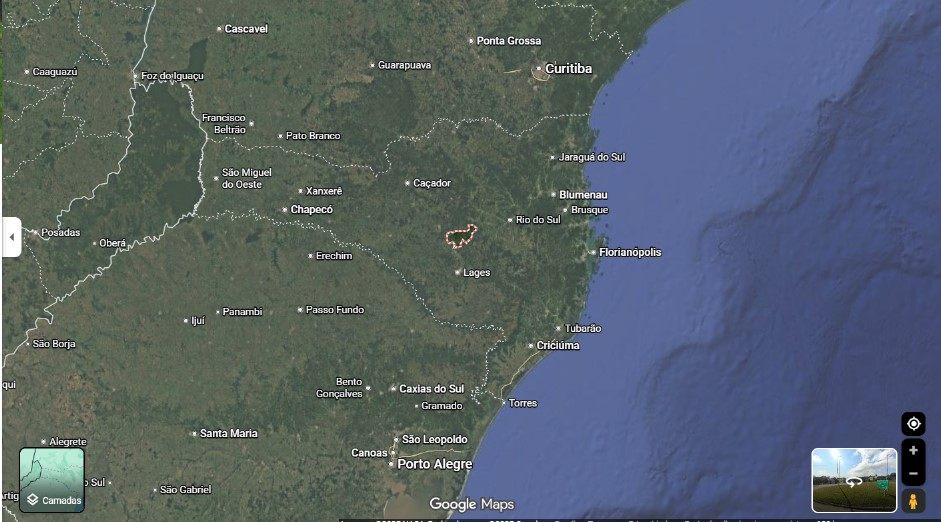
\includegraphics[width=0.9\textwidth]{mapa-ponte-alta.jpg}

\begin{minipage}{0.9\textwidth}
    \setlength{\parindent}{1em}
    \raggedright
    Fonte: Elaborado pelos autores (2025)
\end{minipage}

\end{figuraabnt}

Em suma, a localização e as características físico-ambientais da Fazenda Canoas (topografia ondulada, solos rasos a médios e clima úmido) determinam restrições e oportunidades para a escolha de máquinas e práticas de manejo. Essas condições foram consideradas ao estimar capacidades operacionais e ao propor recomendações técnicas nas seções seguintes.

%figura construções da propriedade

%\begin{figuraabnt}{Área de pastagem}{fig:construcao}
%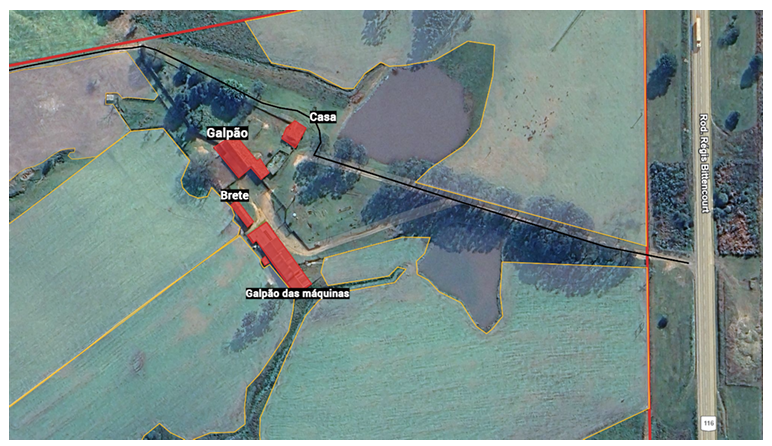
\includegraphics[width=0.9\textwidth]{construcao-je.png}

%\begin{minipage}{0.9\textwidth}
 %   \setlength{\parindent}{1em}
 %   \raggedright
  %  Fonte: O autor (2025)
%\end{minipage}

%\end{figuraabnt}






%seção area topografia
\section{Área, declividade e topografia}
A propriedade tem áreas declivosas com presença de erosão de pastejo nas áreas A10 e A12. Há o manejo com a rotação de animais pelos piquetes, e as áreas de pastagem somam 79,6\,ha totais.

Abaixo, a distribuição das áreas dos piquetes:
\begin{figuraabnt}{Croqui da área}{fig:croqui}
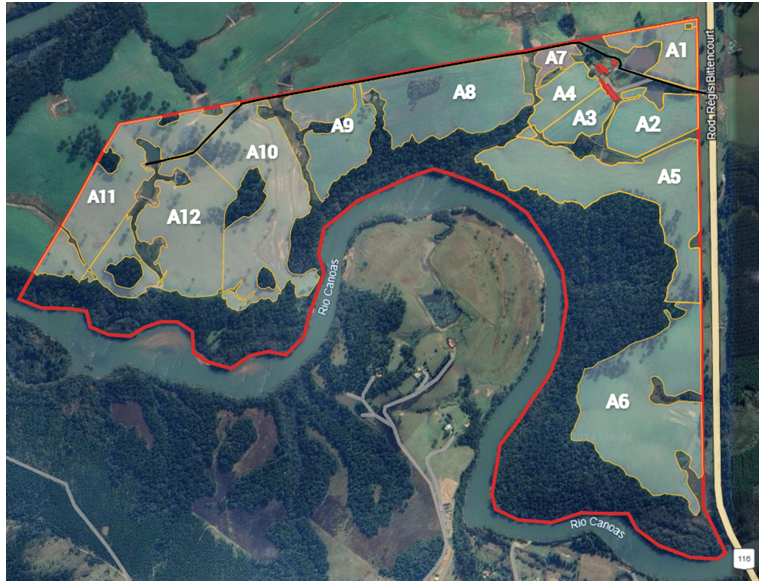
\includegraphics[width=0.9\textwidth]{croqui-je.png}

\begin{minipage}{0.9\textwidth}
    \setlength{\parindent}{1em}
    \raggedright
    Fonte: Elaborado pelos autores (2025)
\end{minipage}

\end{figuraabnt}


% tabela tamanho dos piquetes (ajustada — um pouco maior que a original)
\begin{table}[H]
    \centering
    \caption{Divisão dos piquetes da propriedade}
    \label{tab:piquetes}
    \vspace{0.2cm}
    % aumentar espaçamento das células e envolver em minipage para controlar largura
    \begin{minipage}{0.95\textwidth}
    \centering
    {\small\setlength{\tabcolsep}{14pt}\renewcommand{\arraystretch}{1.15}
    \begin{tabular}{cc|cc}
        
        {Piquete} & \textbf{Área (ha)} & \textbf{Piquete} & \textbf{Área (ha)} \\
        \midrule
        A1 & 2,7  & A7  & 0,8 \\
        A2 & 3,7  & A8  & 8,5 \\
        A3 & 1,8  & A9  & 5,1 \\
        A4 & 2,2  & A10 & 10,9 \\
        A5 & 11,2 & A11 & 8,5 \\
        A6 & 14,2 & A12 & 10,0 \\
        \bottomrule
    \end{tabular}}
    \vspace{0.4em}
    \begin{flushleft}\begin{footnotesize}
        {Fonte:} Dados da propriedade (2025).
    \end{footnotesize}\end{flushleft}
    \end{minipage}
\end{table}

%figura altimetro propriedade


\begin{figuraabnt}{Altímetro da área}{fig:altimetro}
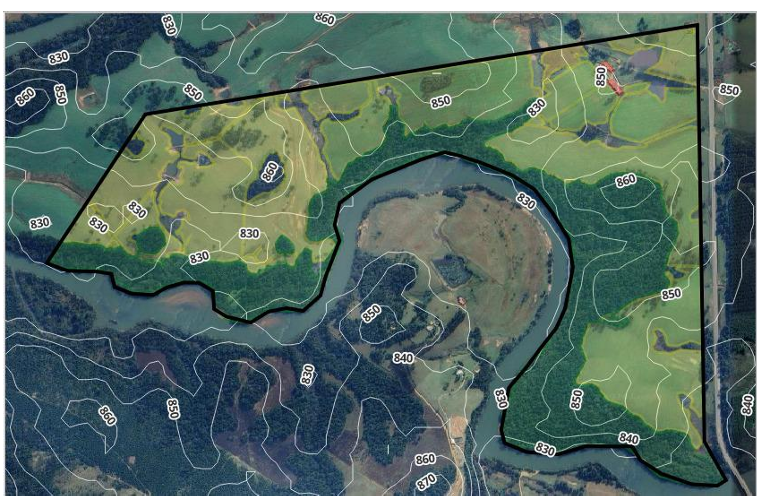
\includegraphics[width=0.9\textwidth]{altimetro-je.png}

\begin{minipage}{0.9\textwidth}
    \setlength{\parindent}{1em}
    \raggedright
    Fonte: Elaborado pelos autores (2025)
\end{minipage}

\end{figuraabnt}

\section{Atividade econômica principal}
A pecuária é a principal atividade da propriedade, essa prática foi iniciada por Antônio Camargo, utilizando animais crioulos (galinhas, porcos, ovelhas e bovinos), consolidando a base histórica e cultural da fazenda.

Atualmente, o uso de máquinas — como dois tratores disponíveis na propriedade — é realizado de forma periódica. Esses equipamentos são empregados principalmente em atividades como a gradagem, realizada duas vezes ao ano para o plantio de pastos, além da distribuição de adubos minerais e orgânicos, otimizando os processos produtivos.

%figura de pastagem
\begin{figuraabnt}{Área de pastagem}{fig:pastagem}
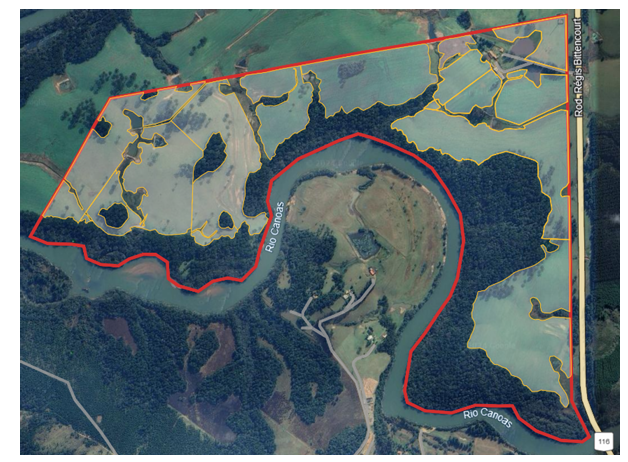
\includegraphics[width=0.9\textwidth]{pastagens-je.png}

\begin{minipage}{0.9\textwidth}
    \setlength{\parindent}{1em}
    \raggedright
   \hspace{0.3cm} Fonte: Elaborado pelos autores (2025)
\end{minipage}

\end{figuraabnt}


\section{Nível de investimento}
Os maquinários utilizados na propriedade foram adquiridos diretamente pelo proprietário, sem recorrer a suporte financeiro externo. O pagamento integral dos equipamentos foi concluído em 2023, consolidando a independência financeira da propriedade em relação a essas aquisições.

No entanto, para suprir as demandas dos cultivos, há empréstimos periódicos realizados junto a cooperativas financeiras, destinados à aquisição de insumos essenciais, como sementes, adubos e corretivos. Esses financiamentos permitem o planejamento eficiente das operações agrícolas, garantindo a continuidade e a qualidade das atividades produtivas.

\section{Época de operações}
O uso mais intensivo dos maquinários ocorre nos meses de novembro a janeiro e de junho a agosto, que correspondem às épocas de plantio das pastagens cultivadas.

\begin{itemize}
    \item \textbf{Equipamentos da prefeitura:} O distribuidor de calcário e adubo orgânico seco é utilizado a cada 1 ou 2 anos em certos piquetes.
    \item \textbf{Preparo do solo:} O uso da grade é destinado à abertura do solo e, posteriormente, para a cobertura da semente.
    \item \textbf{Adubação:} O uso do distribuidor \textit{TRITON-ROTAX TR904 MD650} é para lanço de ureia 45 dias após o plantio, e posterior ao segundo pastoreio para um melhor rebrote do pasto.
\end{itemize}


\begin{figuraabnt}{Gráfico Gantt}{fig:gantt}
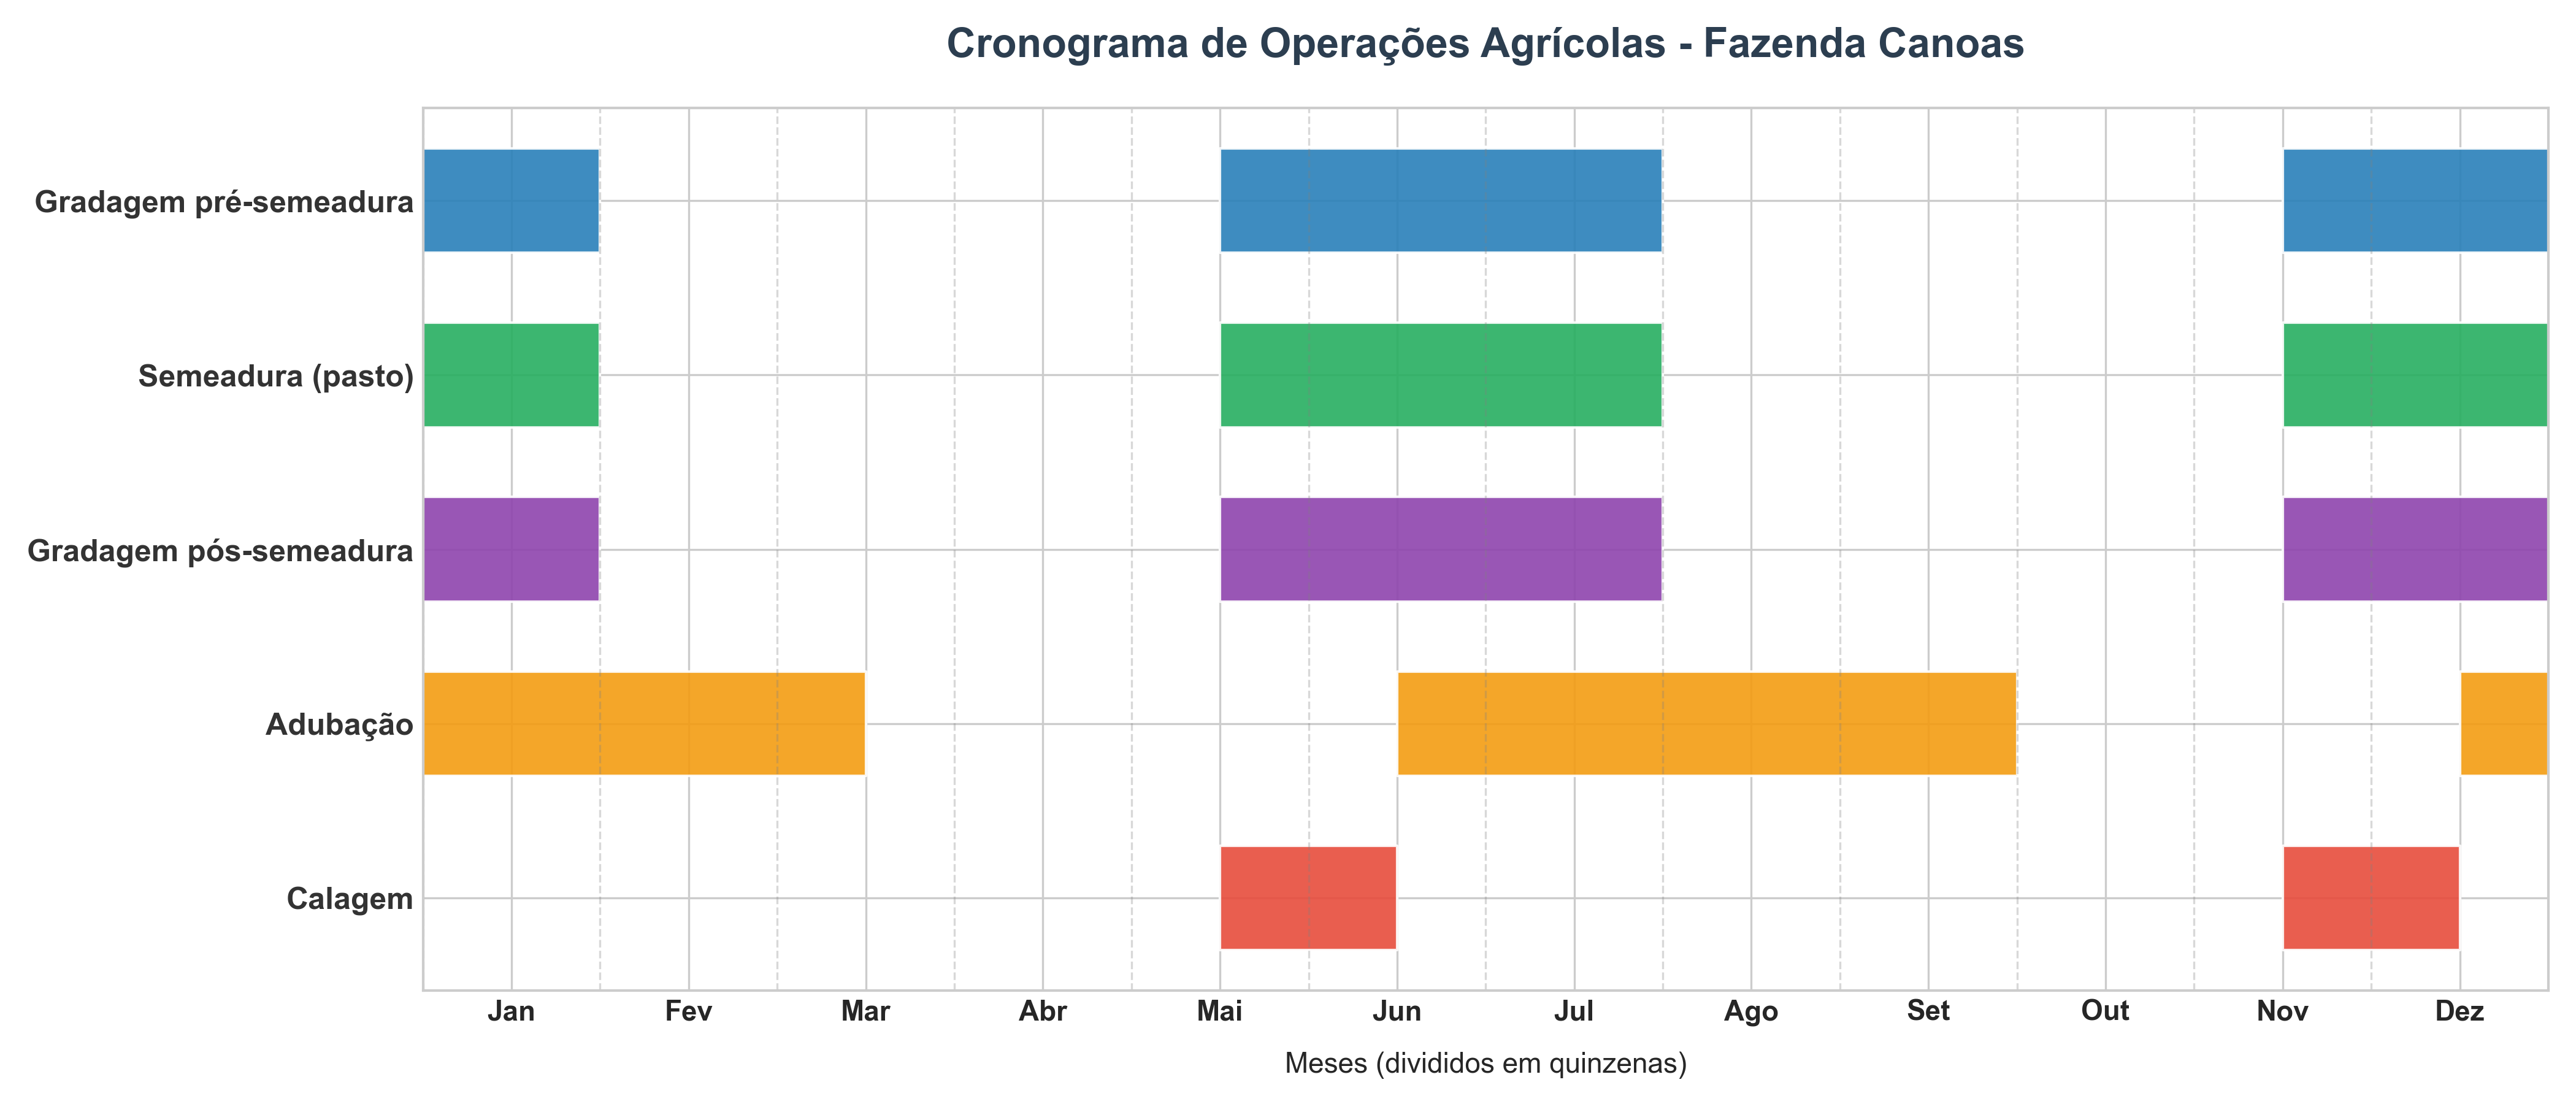
\includegraphics[width=1\textwidth]{grafico_gantt_mecanizacao.png}
\begin{minipage}{0.9\textwidth}
    \setlength{\parindent}{1em}
    \raggedright
    Fonte: Elaborado pelos autores (2025)
\end{minipage}
\end{figuraabnt}


\section{Objetivos específicos}
\begin{itemize}
    \item Verificar o estado das máquinas e sua adequação aos usos da propriedade, identificando excesso ou faltas que possam impactar as eficiências e produtividade.
    \item Identificar possíveis tecnologias que possam contribuir para o aumento da eficiência e redução dos custos operacionais.
    \item Fornecer um relatório detalhado das épocas de operações e capacidade operacional com base nos maquinários e implementos que a propriedade possui.
\end{itemize}




\chapter{Inventário do maquinário}

O levantamento dos equipamentos disponíveis na Fazenda Canoas permitiu a elaboração de um inventário detalhado, visando identificar a capacidade operacional instalada. A Tabela \ref{tab:inventario-geral} resume os principais tratores e implementos identificados, relacionando suas potências nominais e principais finalidades no sistema produtivo.

% Tabela inventario maquinario
\begin{table}[H]
\centering
\caption{Inventário do maquinário e implementos agrícolas da propriedade Fazenda Canoas.}
\label{tab:inventario-geral}
\resizebox{\textwidth}{!}{ % Ajusta a tabela à largura da página
\begin{tabular}{lllll}
\toprule
\textbf{Equipamento} & \textbf{Modelo} & \textbf{Ano} & \textbf{Potência (cv)} & \textbf{Uso principal} \\
\midrule
Trator & LS PLUS 100 & 2017 & 103 cv & Preparo de solo, distribuição \\
Trator & LS PLUS 80 & 2015 & 75 cv & Preparo de solo, distribuição \\
Grade Niveladora & Tatu GNL (28 discos) & -- & (Req: 70-75 cv) & Gradagem \\
Grade & Baldan SPR (28 discos) & -- & (Req: 65-70 cv) & Gradagem \\
Distribuidor Rotativo & TRITON-ROTAX TR904 & -- & -- & Semeadura e Adubação \\
\bottomrule
\end{tabular}}
\end{table}

\section{Implementos para preparo de solo}

Na propriedade, o sistema de manejo de solo predominante é o preparo periódico. Diferente do preparo convencional completo (aração seguida de gradagem), aqui utiliza-se a grade niveladora como implemento principal, tanto para o destorroamento e nivelamento superficial quanto para a incorporação de sementes de forrageiras distribuídas a lanço.

Esta prática é comum na formação de pastagens, mas exige monitoramento técnico. Segundo \citeonline{bauer2019p1}, o uso sistemático de grades na mesma profundidade pode favorecer a formação de uma camada compactada subsuperficial conhecida como ``pé-de-grade'', que prejudica a infiltração de água e o desenvolvimento radicular.

Para a execução destas operações, a propriedade conta com grades niveladoras da marca Baldan, conforme ilustrado na Figura \ref{fig:baldan}. As especificações técnicas detalhadas deste implemento, incluindo a profundidade de corte e a demanda de potência, estão descritas na Tabela \ref{tab:grade-tatu}.

\begin{figuraabnt}{Grade Niveladora Baldan}{fig:baldan}
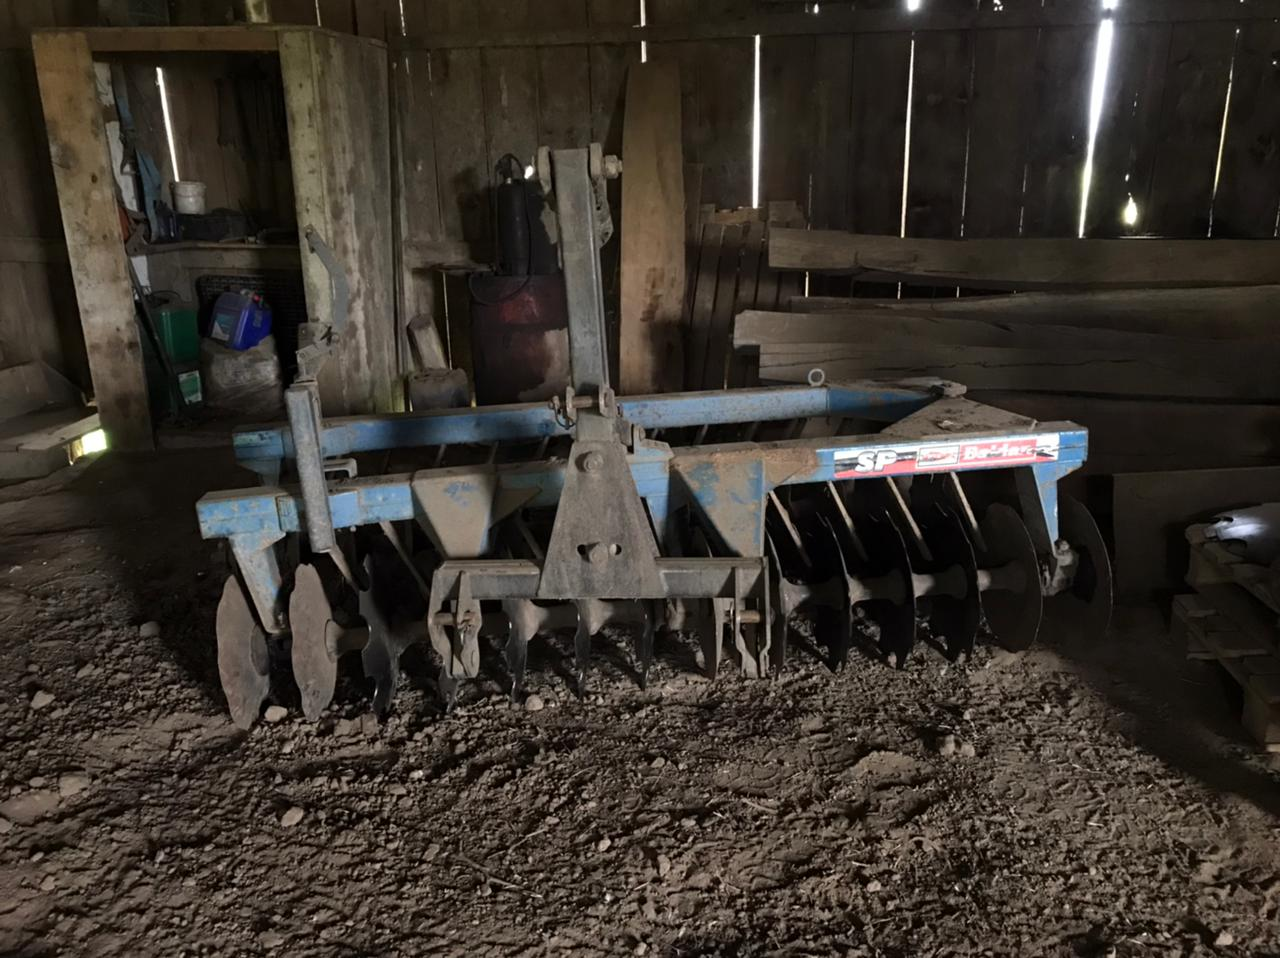
\includegraphics[width=0.75\textwidth]{grade-tatu.jpg}
\begin{minipage}{0.9\textwidth}
    \setlength{\parindent}{1em}
    \raggedright
    Fonte: Elaborado pelos autores (2025)
\end{minipage}
\end{figuraabnt}

\begin{table}[h!]
    \centering
    \caption{Especificações Técnicas - Grade Niveladora Baldan}
    \label{tab:grade-tatu}
    \vspace{0.1cm}
    \begin{tabular}{ll}
        \toprule
        \textbf{Parâmetro} & \textbf{Especificação} \\
        \midrule
        Modelo & GNL (Grade Niveladora Leve) \\
        Tipo de Acoplamento & Barra de Tração \\
        Quantidade de Discos & 28 discos (2 seções) \\
        Diâmetro do Eixo & 31,75\,mm ($1\frac{1}{4}$") \\
        Profundidade de Corte & 60 a 120\,mm \\
        Velocidade de Trabalho & 9 a 12\,km/h \\
        \midrule
        \textit{Componentes Internos} & \\
        Mancais (Comprimento) & 182\,mm \\
        Mancais (Tipo) & Atrito (MA), Graxa (CM) ou Duromark (DM) \\
        Separadores (Comp.) & 167\,mm (Fundido) \\
        \bottomrule
    \end{tabular}
    \vspace{0.1cm}
    \begin{footnotesize}
        \begin{flushleft}
            Fonte: Dados da propriedade / Manual do fabricante.
        \end{flushleft}
    \end{footnotesize}
\end{table}


\section{Fontes de potência (tratores)}

A frota de tratores é composta por dois modelos da fabricante LS Tractor. O equipamento de maior porte, utilizado para as operações que demandam maior força de tração, é o modelo LS PLUS 100 (Figura \ref{fig:trator-maior}). Suas características técnicas, como motorização e escalonamento de marchas, são apresentadas na Tabela \ref{tab:trator-ls}.

\begin{figuraabnt}{Trator LS PLUS 100}{fig:trator-maior}
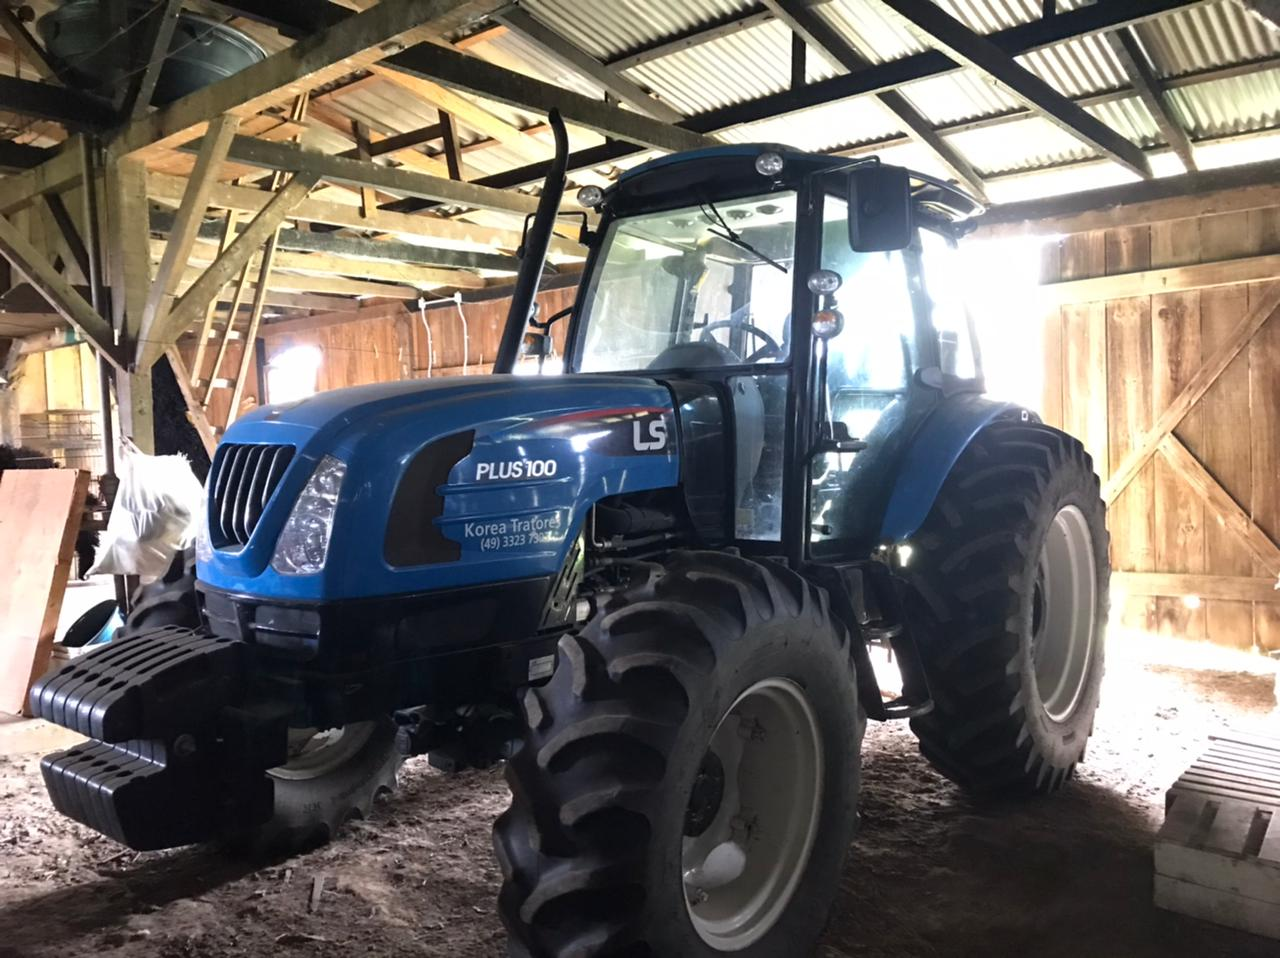
\includegraphics[width=0.75\textwidth]{trator-maior.jpg}
\begin{minipage}{0.9\textwidth}
    \setlength{\parindent}{1em}
    \raggedright
    Fonte: Elaborado pelos autores (2025)
\end{minipage}
\end{figuraabnt}

O principal trator da propriedade é o modelo LS PLUS 100, conforme ilustrado na Figura \ref{fig:trator-maior}. Trata-se de um trator de porte médio, adequado para as operações de preparo de solo e distribuição de insumos na fazenda. A Tabela \ref{tab:trator-ls} detalha suas especificações técnicas, destacando aspectos como potência, torque e características do motor e transmissão.

\begin{table}[H]
    \centering
    \caption{Especificações Técnicas - Trator LS PLUS 100 (Ano 2017)}
    \label{tab:trator-ls}
    \vspace{0.1cm}
    \begin{tabular}{ll}
        \toprule
        \textbf{Parâmetro} & \textbf{Especificação} \\
        \midrule
        Modelo & LS PLUS 100 (103\,cv) \\
        \midrule
        \textit{Pesos e Lastragem} & \\
        Peso Cabinado & 3910\,kg \\
        Suporte de Peso Frontal & 70\,kg \\
        Pesos Frontais & $10 \times 40$\,kg (400\,kg totais) \\
        Pesos Traseiros & $2 \times 90$\,kg (180\,kg totais) \\
        \midrule
        \textit{Motor (Modelo TD229-4)} & \\
        Tipo & Diesel, 4 cil. vertical, refrig. a água \\
        Deslocamento & 3922\,cc ($102 \times 120$\,mm) \\
        Potência Máxima & 75,7\,kW (103\,ps) a 2400\,rpm \\
        Torque Máximo & 372\,N.m a 1400\,rpm \\
        Rotação de Trabalho & 750 a 2630\,rpm \\
        Ordem de Injeção & 1-3-4-2 \\
        \midrule
        \textit{Transmissão} & \\
        Configuração de Marchas & F12$\times$R12 / F20$\times$R20 \\
        Embreagem Principal & Placa Única Seca \\
        Reversor & Tipo Inversor Sincronizado \\
        Bloqueio do Diferencial & Eletro-Hidráulico \\
        \midrule
        \textit{Sistemas Auxiliares} & \\
        Bomba Injetora & Tipo Distribuição (Reg. Centrífuga) \\
        Sistema de Lubrificação & Circulação Forçada (Bomba de Engrenagem) \\
        Arrefecimento & Bomba Centrífuga com Termostato \\
        Filtros (Ar/Comb./Óleo) & Seco / Cartucho Substituível \\
        \bottomrule
    \end{tabular}
    \vspace{0.1cm}
    \begin{footnotesize}
        \begin{flushleft}
            Fonte: Dados da propriedade / Manual do fabricante.
        \end{flushleft}
    \end{footnotesize}
\end{table}

Como fonte de potência auxiliar, a propriedade conta com o modelo LS PLUS 80. Conforme ilustrado na Figura \ref{fig:trator80}, trata-se de um trator de porte médio. A Tabela \ref{tab:trator-ls80} detalha suas especificações, destacando-se a diferença de potência e torque em relação ao modelo maior.



  
\begin{figuraabnt}{Vista lateral e acoplamento do Trator LS PLUS 80}{fig:trator80}
% aumentar espaço entre o título da figura e as imagens
\vspace{1em}
% duas imagens lado a lado, alinhadas verticalmente ao centro e com altura igual
\begin{minipage}[c]{0.48\textwidth}
    \centering
    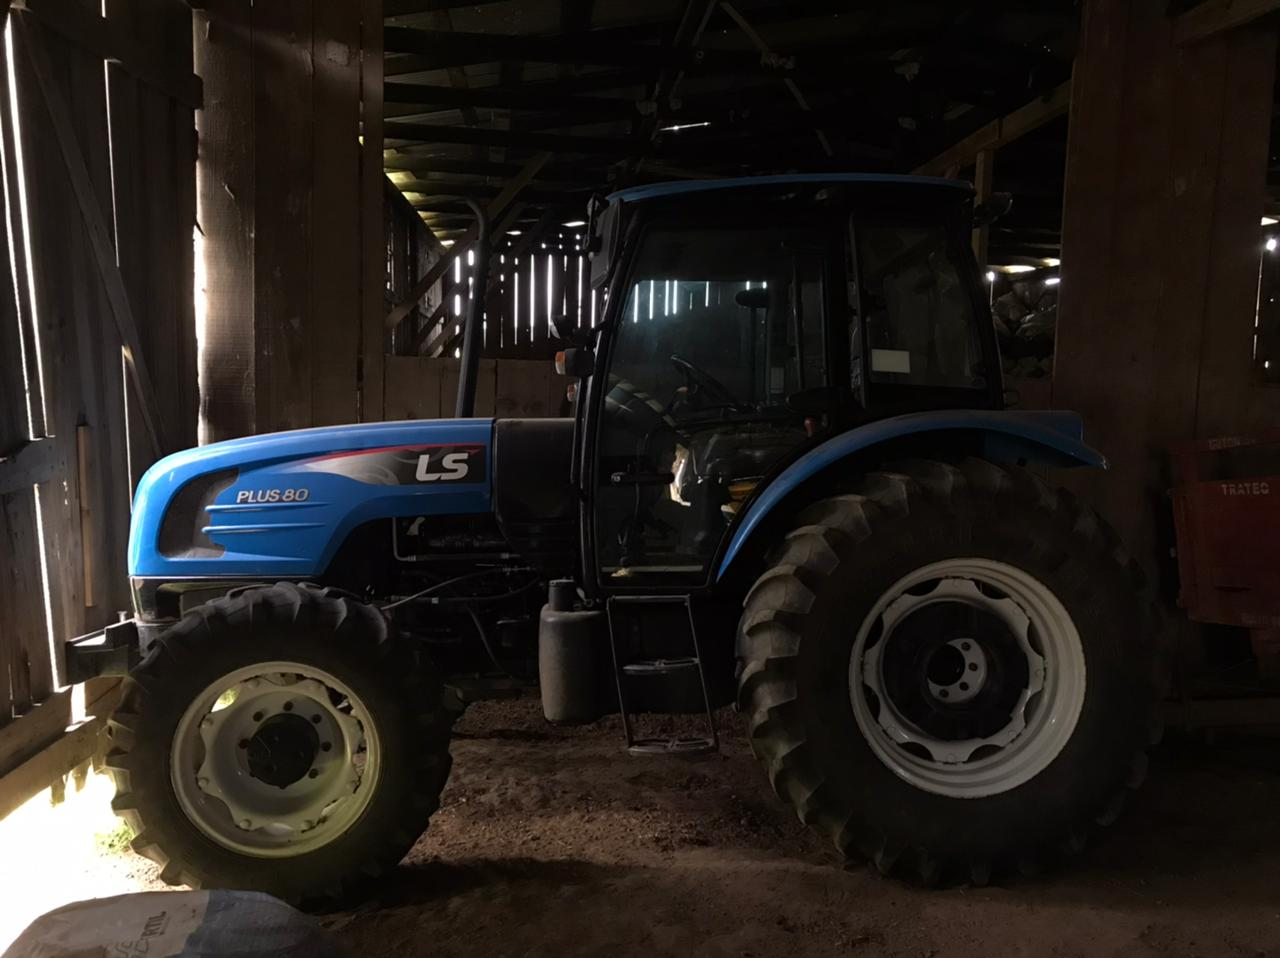
\includegraphics[height=5.5cm]{trator-menor.jpg}
    \\[0.3em]\small (a) Vista lateral do trator
\end{minipage}\hfill
\begin{minipage}[c]{0.48\textwidth}
    \centering
        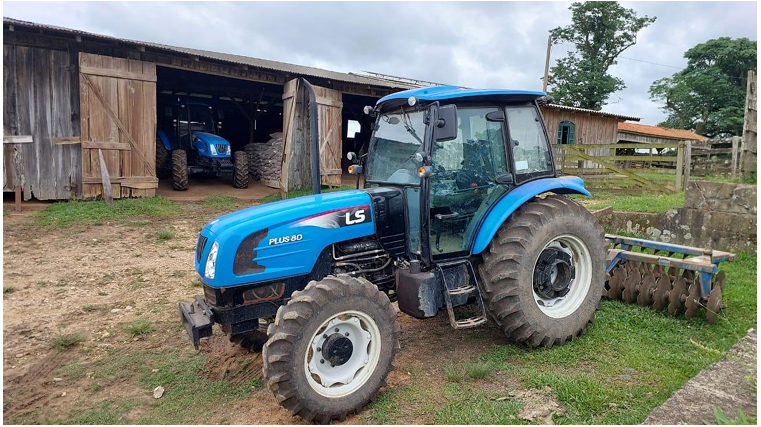
\includegraphics[height=5.5cm,width=1.2\linewidth,keepaspectratio]{trator80-acoplado.png}
    \\[0.3em]\small (b) Trator com implemento acoplado
\end{minipage}

\vspace{0.6em}
\begin{minipage}{0.9\textwidth}
        \setlength{\parindent}{1em}
        \raggedright
        Fonte: Elaborado pelos autores (2025)
\end{minipage}
\end{figuraabnt}

\begin{table}[H]
    \centering
    \caption{Especificações Técnicas - Trator LS PLUS 80 (Ano 2015)}
    \label{tab:trator-ls80}
    \vspace{0.1cm}
    \begin{tabular}{ll}
        \toprule
        \textbf{Parâmetro} & \textbf{Especificação} \\
        \midrule
        Modelo & LS PLUS 80 (Ano 2015) \\
        \midrule
        \textit{Pesos e Lastragem} & \\
        Peso Cabinado & 3680\,kg \\
        Suporte de Peso Frontal & 70\,kg \\
        Pesos Frontais & $10 \times 40$\,kg (400\,kg totais) \\
        Pesos Traseiros & $2 \times 90$\,kg (180\,kg totais) \\
        \midrule
        \textit{Motor (Modelo D222-4)} & \\
        Tipo & Diesel, 4 cil. vertical, refrig. a água \\
        Deslocamento & 3922\,cc ($102 \times 120$\,mm) \\
        Potência & 55,1\,kW (75\,ps) a 2400\,rpm \\
        Torque Máximo & 264\,N.m a 1400\,rpm \\
        Rotação de Trabalho & 750 a 2630\,rpm \\
        Ordem de Injeção & 1-3-4-2 \\
        \midrule
        \textit{Transmissão} & \\
        Configuração de Marchas & F12$\times$R12 / F20$\times$R20 \\
        Embreagem Principal & Placa Única Seca \\
        Reversor & Tipo Inversor Sincronizado \\
        Bloqueio do Diferencial & Eletro-Hidráulico \\
        \midrule
        \textit{Sistemas Auxiliares} & \\
        Bomba Injetora & Tipo Distribuição (Reg. Centrífuga) \\
        Sistema de Lubrificação & Circulação Forçada (Bomba de Engrenagem) \\
        Arrefecimento & Bomba Centrífuga com Termostato \\
        Filtros (Ar/Comb./Óleo) & Seco / Cartucho Substituível \\
        \bottomrule
    \end{tabular}
    \vspace{0.1cm}
    \begin{footnotesize}
        \begin{flushleft}
            Fonte: Dados da propriedade / Manual do fabricante.
        \end{flushleft}
    \end{footnotesize}
\end{table}

\section{Distribuição de sólidos}

Para a aplicação de fertilizantes e sementes, utiliza-se o distribuidor rotativo apresentado na Figura \ref{fig:triton}. A Tabela \ref{tab:distribuidor-triton} exibe as características operacionais do equipamento, incluindo sua capacidade volumétrica e largura efetiva de trabalho, parâmetros essenciais para o cálculo de rendimento operacional.

\begin{figuraabnt}{Distribuidor Rotativo TRITON-ROTAX}{fig:triton}
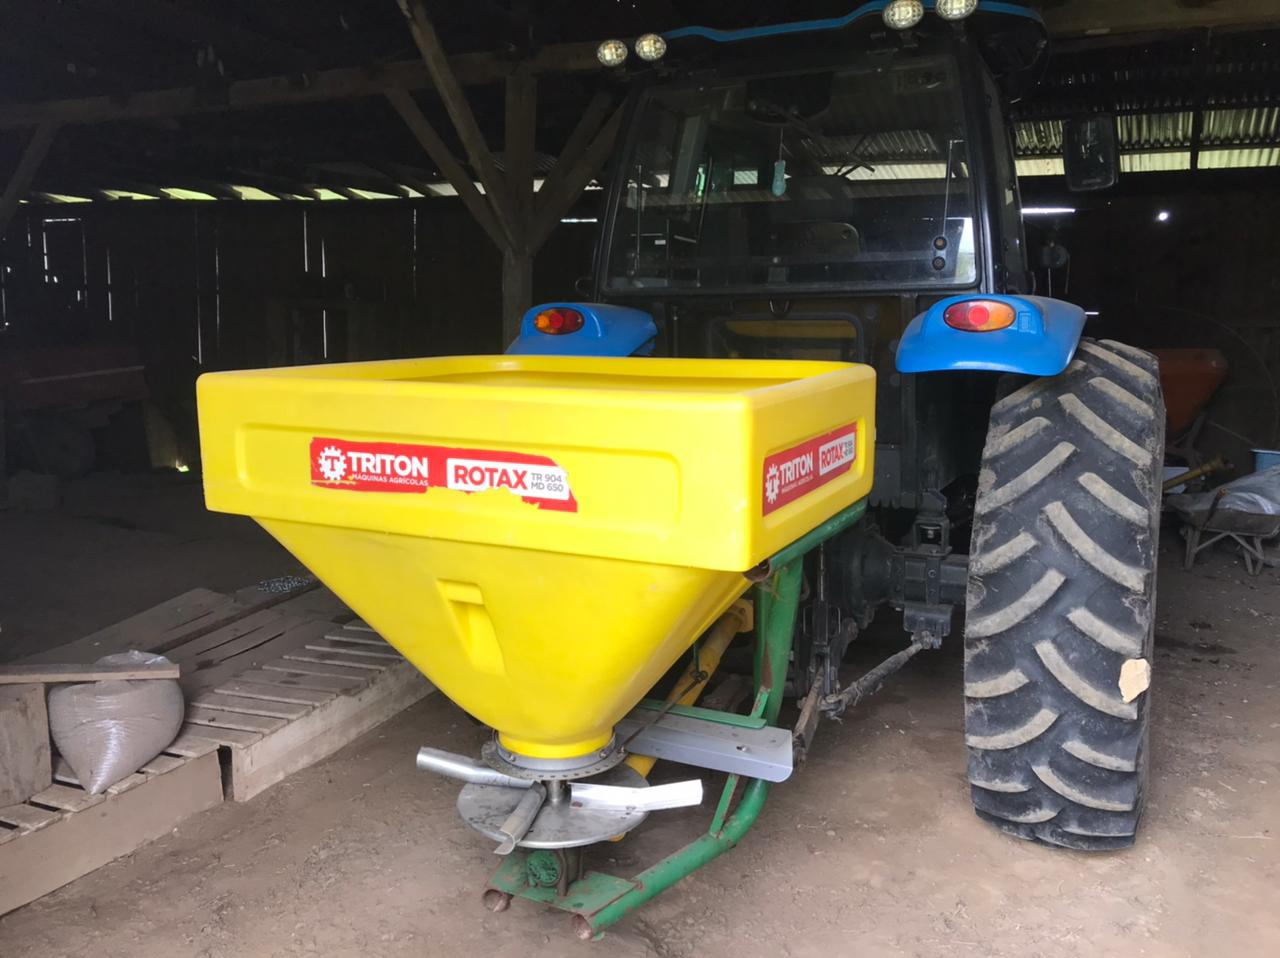
\includegraphics[width=0.75\textwidth]{distribuidor-triton.jpg}
\begin{minipage}{0.9\textwidth}
    \setlength{\parindent}{1em}
    \raggedright
    Fonte: Elaborado pelos autores (2025)
\end{minipage}
\end{figuraabnt}

\begin{table}[h!]
    \centering
    \caption{Especificações Técnicas - Distribuidor Rotativo (TRITON-ROTAX TR904 MD650)}
    \label{tab:distribuidor-triton}
    \vspace{0.1cm}
    \begin{tabular}{ll}
        \toprule
        \textbf{Parâmetro} & \textbf{Especificação} \\
        \midrule
        Modelo & TRITON-ROTAX TR904 MD650 \\
        Sistema de Engate & 3 pontos (Pinos Cat. I e II) \\
        Rotação na TDP & 540\,rpm \\
        \midrule
        \textit{Capacidade e Desempenho} & \\
        Capacidade do Reservatório & 1300\,L \\
        Largura de Trabalho Efetiva & 18 a 38\,m \\
        Peso (Vazio) & 180\,kg \\
        \midrule
        \textit{Dimensões} & \\
        Altura & 130\,cm \\
        Largura & 225\,cm \\
        Comprimento & 145\,cm \\
        \bottomrule
    \end{tabular}
    \vspace{0.1cm}
    \begin{footnotesize}
        \begin{flushleft}
            Fonte: Dados da propriedade / Manual do fabricante.
        \end{flushleft}
    \end{footnotesize}
\end{table}

%ultimo gemi
\chapter{Análise de desempenho operacional e Energético}

A escolha e o dimensionamento das máquinas agrícolas devem ser realizados de forma racional, adequando-se ao sistema de produção e às características econômicas do empreendimento. Segundo \citeonline{bauer2019p1}, o sistema mecanizado pode representar de 20 a 40\% dos custos de produção, tornando essencial o estudo das operações para racionalizar o uso das máquinas e minimizar custos sem afetar a produtividade.

\section{Fundamentação teórica e metodologia}

Para o diagnóstico da capacidade de trabalho do parque de máquinas da Fazenda Canoas, utilizou-se a metodologia de Capacidade Operacional, que permite estimar a quantidade de trabalho executada num determinado período de tempo. Conforme descrito por \citeonline{bauer2019p1}, é necessário distinguir o potencial teórico da máquina de sua realidade no campo.

\subsection{Capacidade de campo teórica ($CcT$)}
Esta métrica representa o potencial máximo de trabalho da máquina, assumindo que ela utilize 100\% de sua largura de corte e opere 100\% do tempo sem interrupções. É um dado de referência calculado pela Equação \ref{eq:cct}:

\begin{equation} \label{eq:cct}
    CcT = \frac{L \times V}{10}
\end{equation}

\noindent Onde:\\
$CcT$ = Capacidade de campo teórica (ha/h);\\
$L$ = Largura de trabalho do implemento (m);\\
$V$ = Velocidade de deslocamento (km/h);\\
$10$ = Fator de conversão de unidades.

\subsection{Eficiência de campo ($Ef$) e capacidade operacional ($CcO$)}
Na prática agrícola, ocorrem perdas de tempo devido a manobras de cabeceira, reabastecimentos, regulagens e embuchamentos. \citeonline{bauer2019p1} definem a Eficiência de Campo ($Ef$) como a relação entre o tempo efetivamente trabalhado e o tempo total da máquina na lavoura.

A Capacidade de Campo Operacional ($CcO$), que é o valor real utilizado para o planejamento, é obtida corrigindo-se a capacidade teórica pela eficiência, conforme Equação \ref{eq:cco}:

\begin{equation} \label{eq:cco}
    CcO = \frac{L \times V \times Ef}{10}
\end{equation}

\noindent Onde $Ef$ é a eficiência de campo (decimal). Para este estudo, adotaram-se índices de eficiência conservadores (0,75 a 0,85) para garantir que o planejamento de tempo não seja subestimado.

\section{Parâmetros dos conjuntos mecanizados}

Com base nos dados coletados em campo (velocidade média de operação e largura útil dos implementos), foram calculados os parâmetros operacionais apresentados na Tabela \ref{tab:parametros_maquinas}.

\begin{table}[H]
    \centering
    \caption{Parâmetros operacionais e eficiência estimada dos conjuntos.}
    \label{tab:parametros_maquinas}
    \vspace{0.1cm}
    \begin{tabular}{lcccccc}
        \toprule
        \textbf{Operação} & \textbf{Implemento} & \textbf{\textit{V}} & \textbf{\textit{L}} & \textbf{$CcT$} & \textbf{$Ef$\textsuperscript{*}} & \textbf{$CcO$} \\
         & & (km/h) & (m) & (ha/h) & (\%) & (ha/h) \\
        \midrule
        Gradagem & Grade Niveladora & 9,0 & 2,35 & 2,12 & 75 & \textbf{1,59} \\
        Distribuição & Distribuidor Rotativo & 6,0 & 7,00 & 4,20 & 80 & \textbf{3,36} \\
        \bottomrule
    \end{tabular}
    \begin{flushleft}\begin{footnotesize}
       Fonte: Autores (2025). \textsuperscript{*}Eficiência estimada considerando geometria dos piquetes e manobras.
    \end{footnotesize}\end{flushleft}
\end{table}

O Tempo Operativo ($TO$), necessário para trabalhar um hectare, é o inverso da capacidade operacional ($TO = 1/CcO$). Este indicador é fundamental para prever quantas horas de trator serão necessárias para cobrir cada piquete.
\begin{itemize}
    \item \textbf{Gradagem:} $TO = 1 / 1,59 = 0,63$ h/ha (aprox. 38 min/ha).
    \item \textbf{Distribuição:} $TO = 1 / 3,36 = 0,30$ h/ha (aprox. 18 min/ha).
\end{itemize}

A proporção de tempo gasto em cada operação é visualizada na Figura \ref{fig:tempo-ope}, que permite compreender rapidamente qual operação demanda maior investimento de horas de máquina. A gradagem, por ser mais exigente em tempo operativo (38 min/ha), concentra a maior parcela do tempo total necessário para a reforma de pastagens, enquanto a distribuição de insumos, sendo mais rápida (18 min/ha), requer menor tempo relativo. Este conhecimento é essencial para o planejamento de mão de obra, disponibilidade de máquinas e gestão das janelas de trabalho.

\begin{figuraabnt}{Tempo por operacao}{fig:tempo-ope}
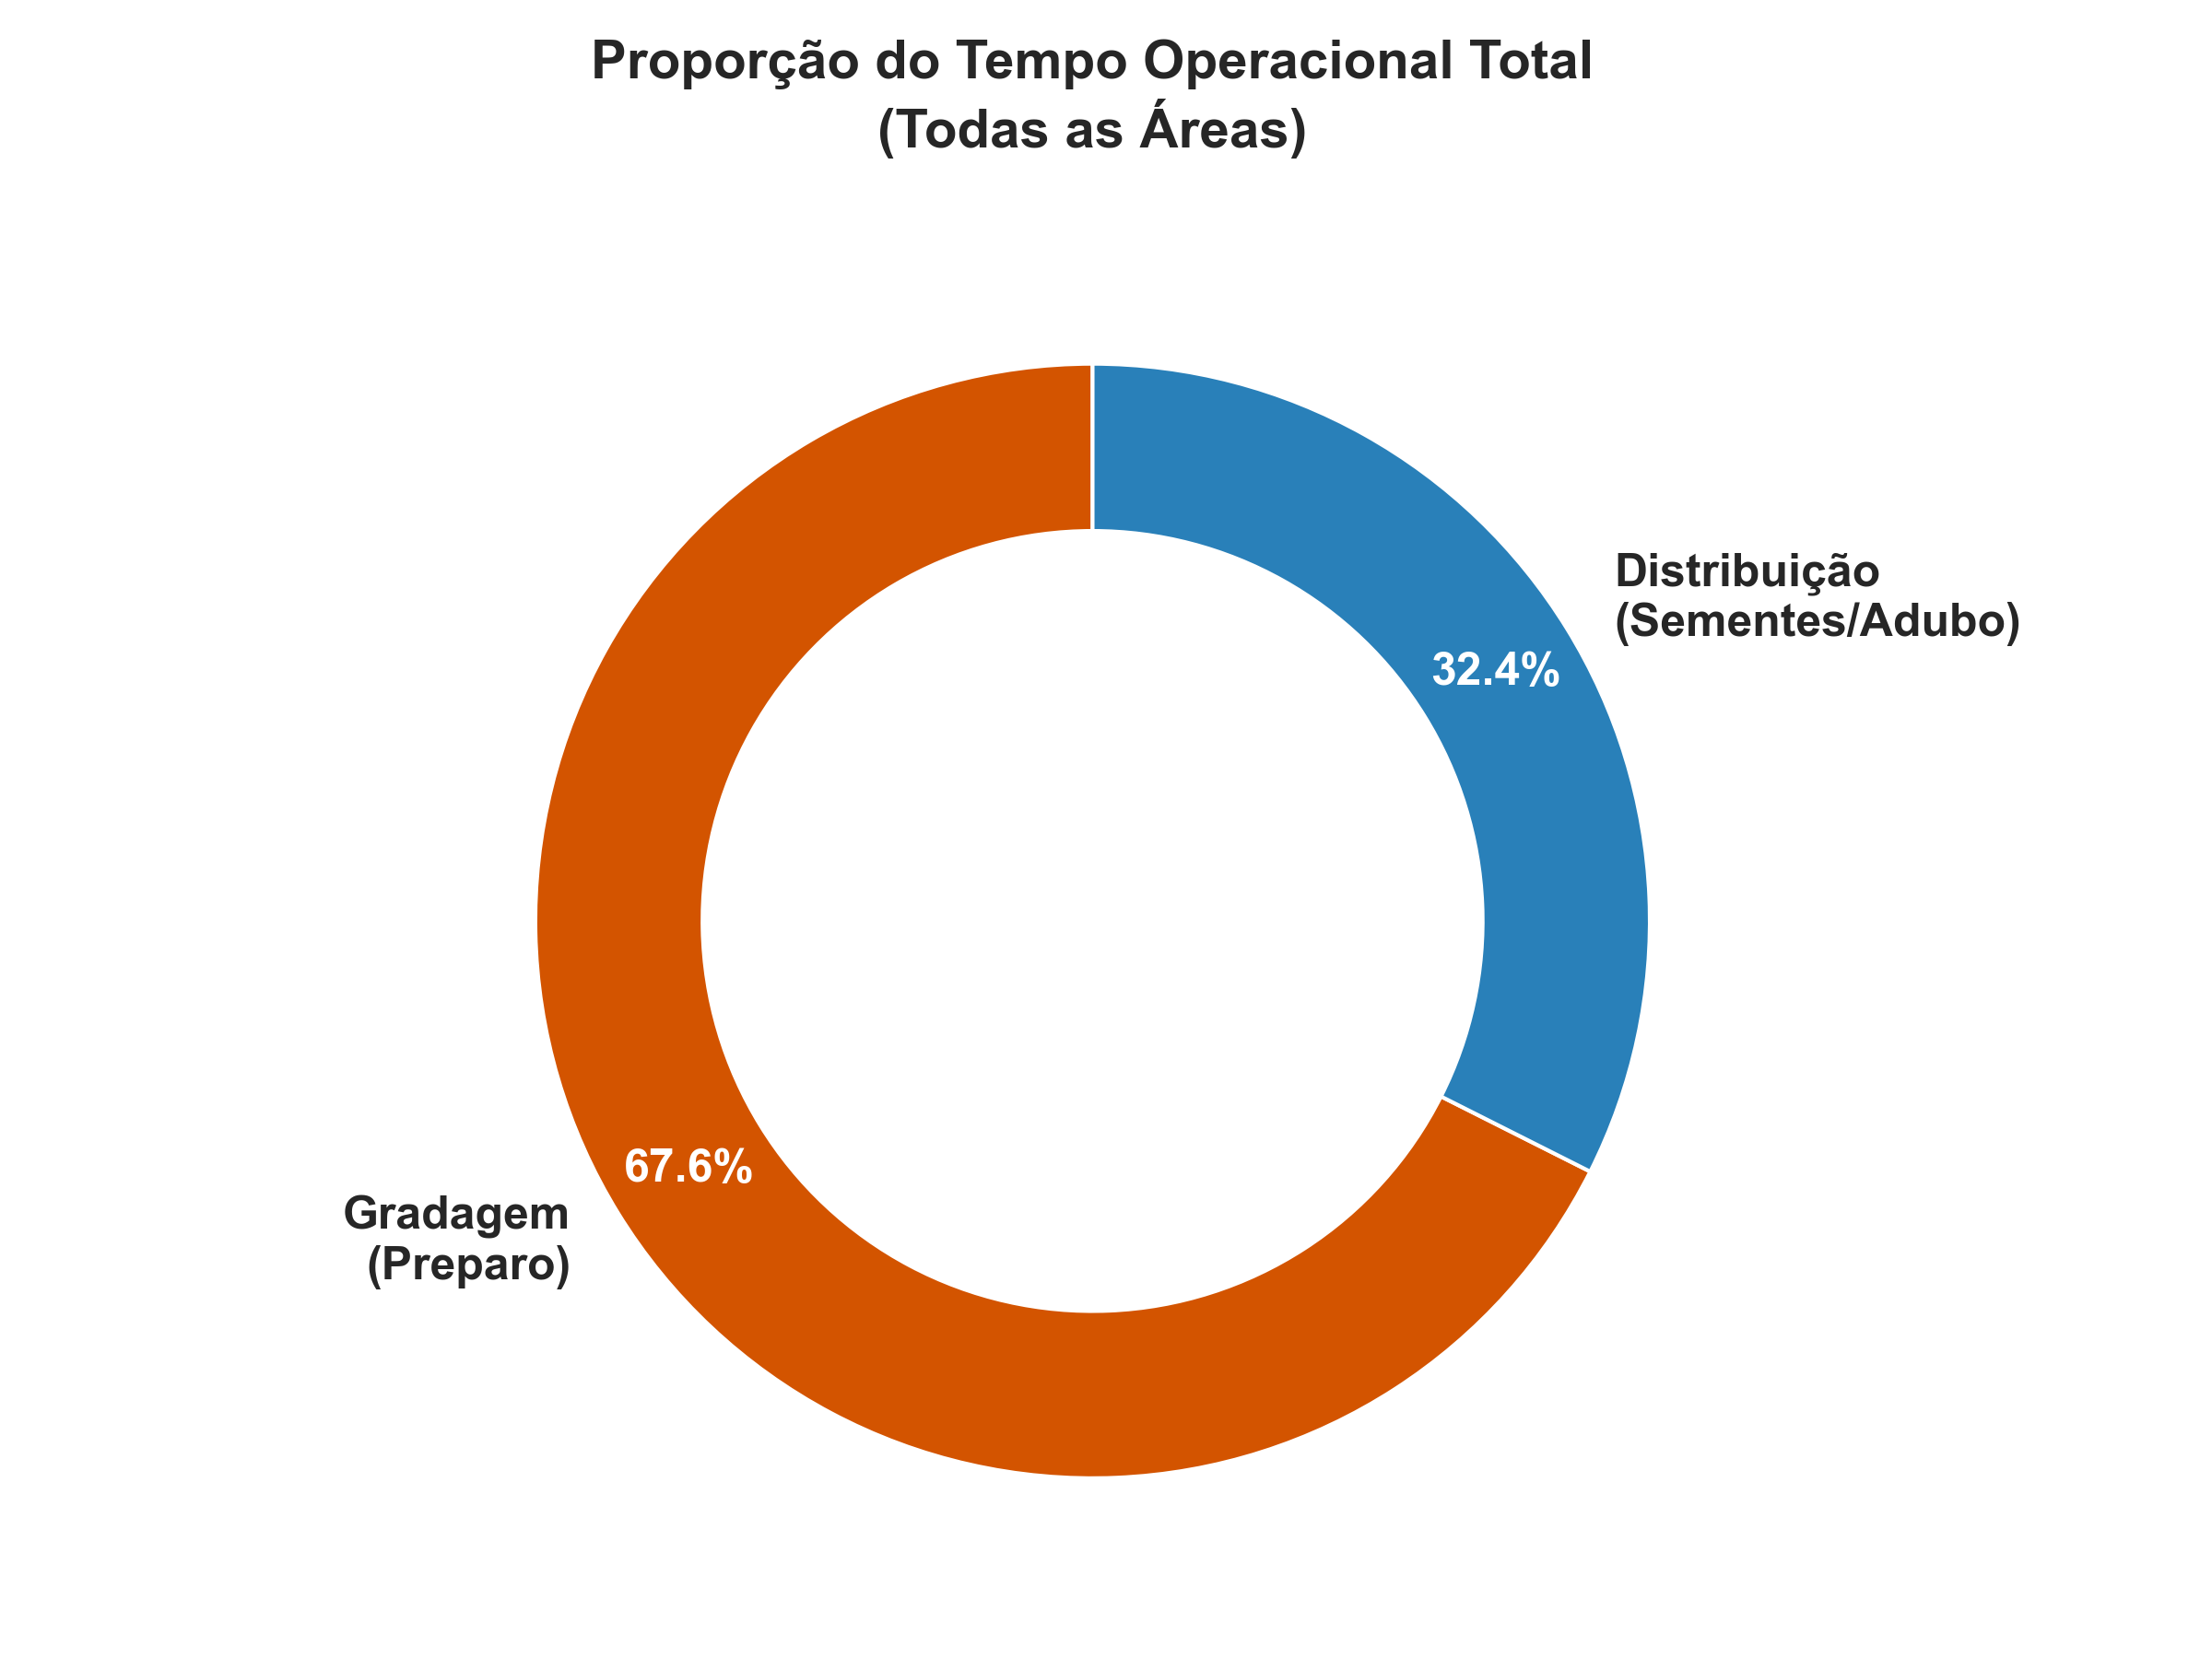
\includegraphics[width=0.75\textwidth]{grafico_proporcao_tempo.png}

\begin{minipage}{0.9\textwidth}
    \setlength{\parindent}{1em}
    \raggedright
    Fonte: Elaborado pelos autores (2025)
\end{minipage}

\end{figuraabnt}
\section{Dimensionamento temporal por piquete}

A Tabela \ref{tab:tempos_piquete} apresenta o tempo estimado para realizar uma operação em cada um dos piquetes produtivos. O cálculo considera a área do piquete multiplicada pelo Tempo Operativo ($TO$), acrescido de um tempo fixo auxiliar ($T_{aux}$) de 5 minutos para deslocamento até as áreas mais distantes (A5, A6 e A7), conforme observado na logística da fazenda.

\begin{table}[H]
    \centering
    \caption{Estimativa de tempo real de trabalho por piquete (por passada).}
    \label{tab:tempos_piquete}
    \vspace{0.1cm}
    \resizebox{\textwidth}{!}{
    \begin{tabular}{cccccc}
        \toprule
        \textbf{Piquete} & \textbf{Área} & \multicolumn{2}{c}{\textbf{Gradagem}} & \multicolumn{2}{c}{\textbf{Distribuição}} \\
        \cmidrule(lr){3-4} \cmidrule(lr){5-6}
         & (ha) & \textbf{Cálculo ($Area \times TO$)} & \textbf{Tempo Total} & \textbf{Cálculo ($Area \times TO$)} & \textbf{Tempo Total} \\
        \midrule
        A3 & 1,8 & $1,8 \times 38$ min & \textbf{1h 08min} & $1,8 \times 18$ min & \textbf{32 min} \\
        A4 & 2,2 & $2,2 \times 38$ min & \textbf{1h 23min} & $2,2 \times 18$ min & \textbf{40 min} \\
        A5 & 11,2 & $11,2 \times 38$ min + $T_{aux}$ & \textbf{7h 10min} & $11,2 \times 18$ min + $T_{aux}$ & \textbf{3h 26min} \\
        A6 & 14,2 & $14,2 \times 38$ min + $T_{aux}$ & \textbf{9h 05min} & $14,2 \times 18$ min + $T_{aux}$ & \textbf{4h 20min} \\
        A7 & 0,8 & $0,8 \times 38$ min + $T_{aux}$ & \textbf{35 min} & $0,8 \times 18$ min + $T_{aux}$ & \textbf{19 min} \\
        \bottomrule
    \end{tabular}}
    \begin{flushleft}\begin{footnotesize}
        Fonte: Autores (2025).
    \end{footnotesize}\end{flushleft}
\end{table}

A distribuição temporal entre os piquetes revela diferenças significativas na demanda de trabalho de máquina, refletindo diretamente a variabilidade de áreas e a necessidade de deslocamentos auxiliares. A Figura \ref{fig:piquete-tempo} apresenta graficamente o tempo total necessário para a reforma completa de cada piquete (considerando 2 passadas de gradagem e 2 de distribuição). Os piquetes maiores (A5 e A6 ) naturalmente demandam maior investimento de horas, enquanto piquetes menores (A3 e A7) requerem menor tempo. Este conhecimento é fundamental para sequenciar as operações, estimar a duração total do ciclo de reforma e priorizar piquetes com maiores restrições de janela operacional devido a condições climáticas.

%figura grafico piquetes tempo
\begin{figuraabnt}{Tempo por piquete}{fig:piquete-tempo}
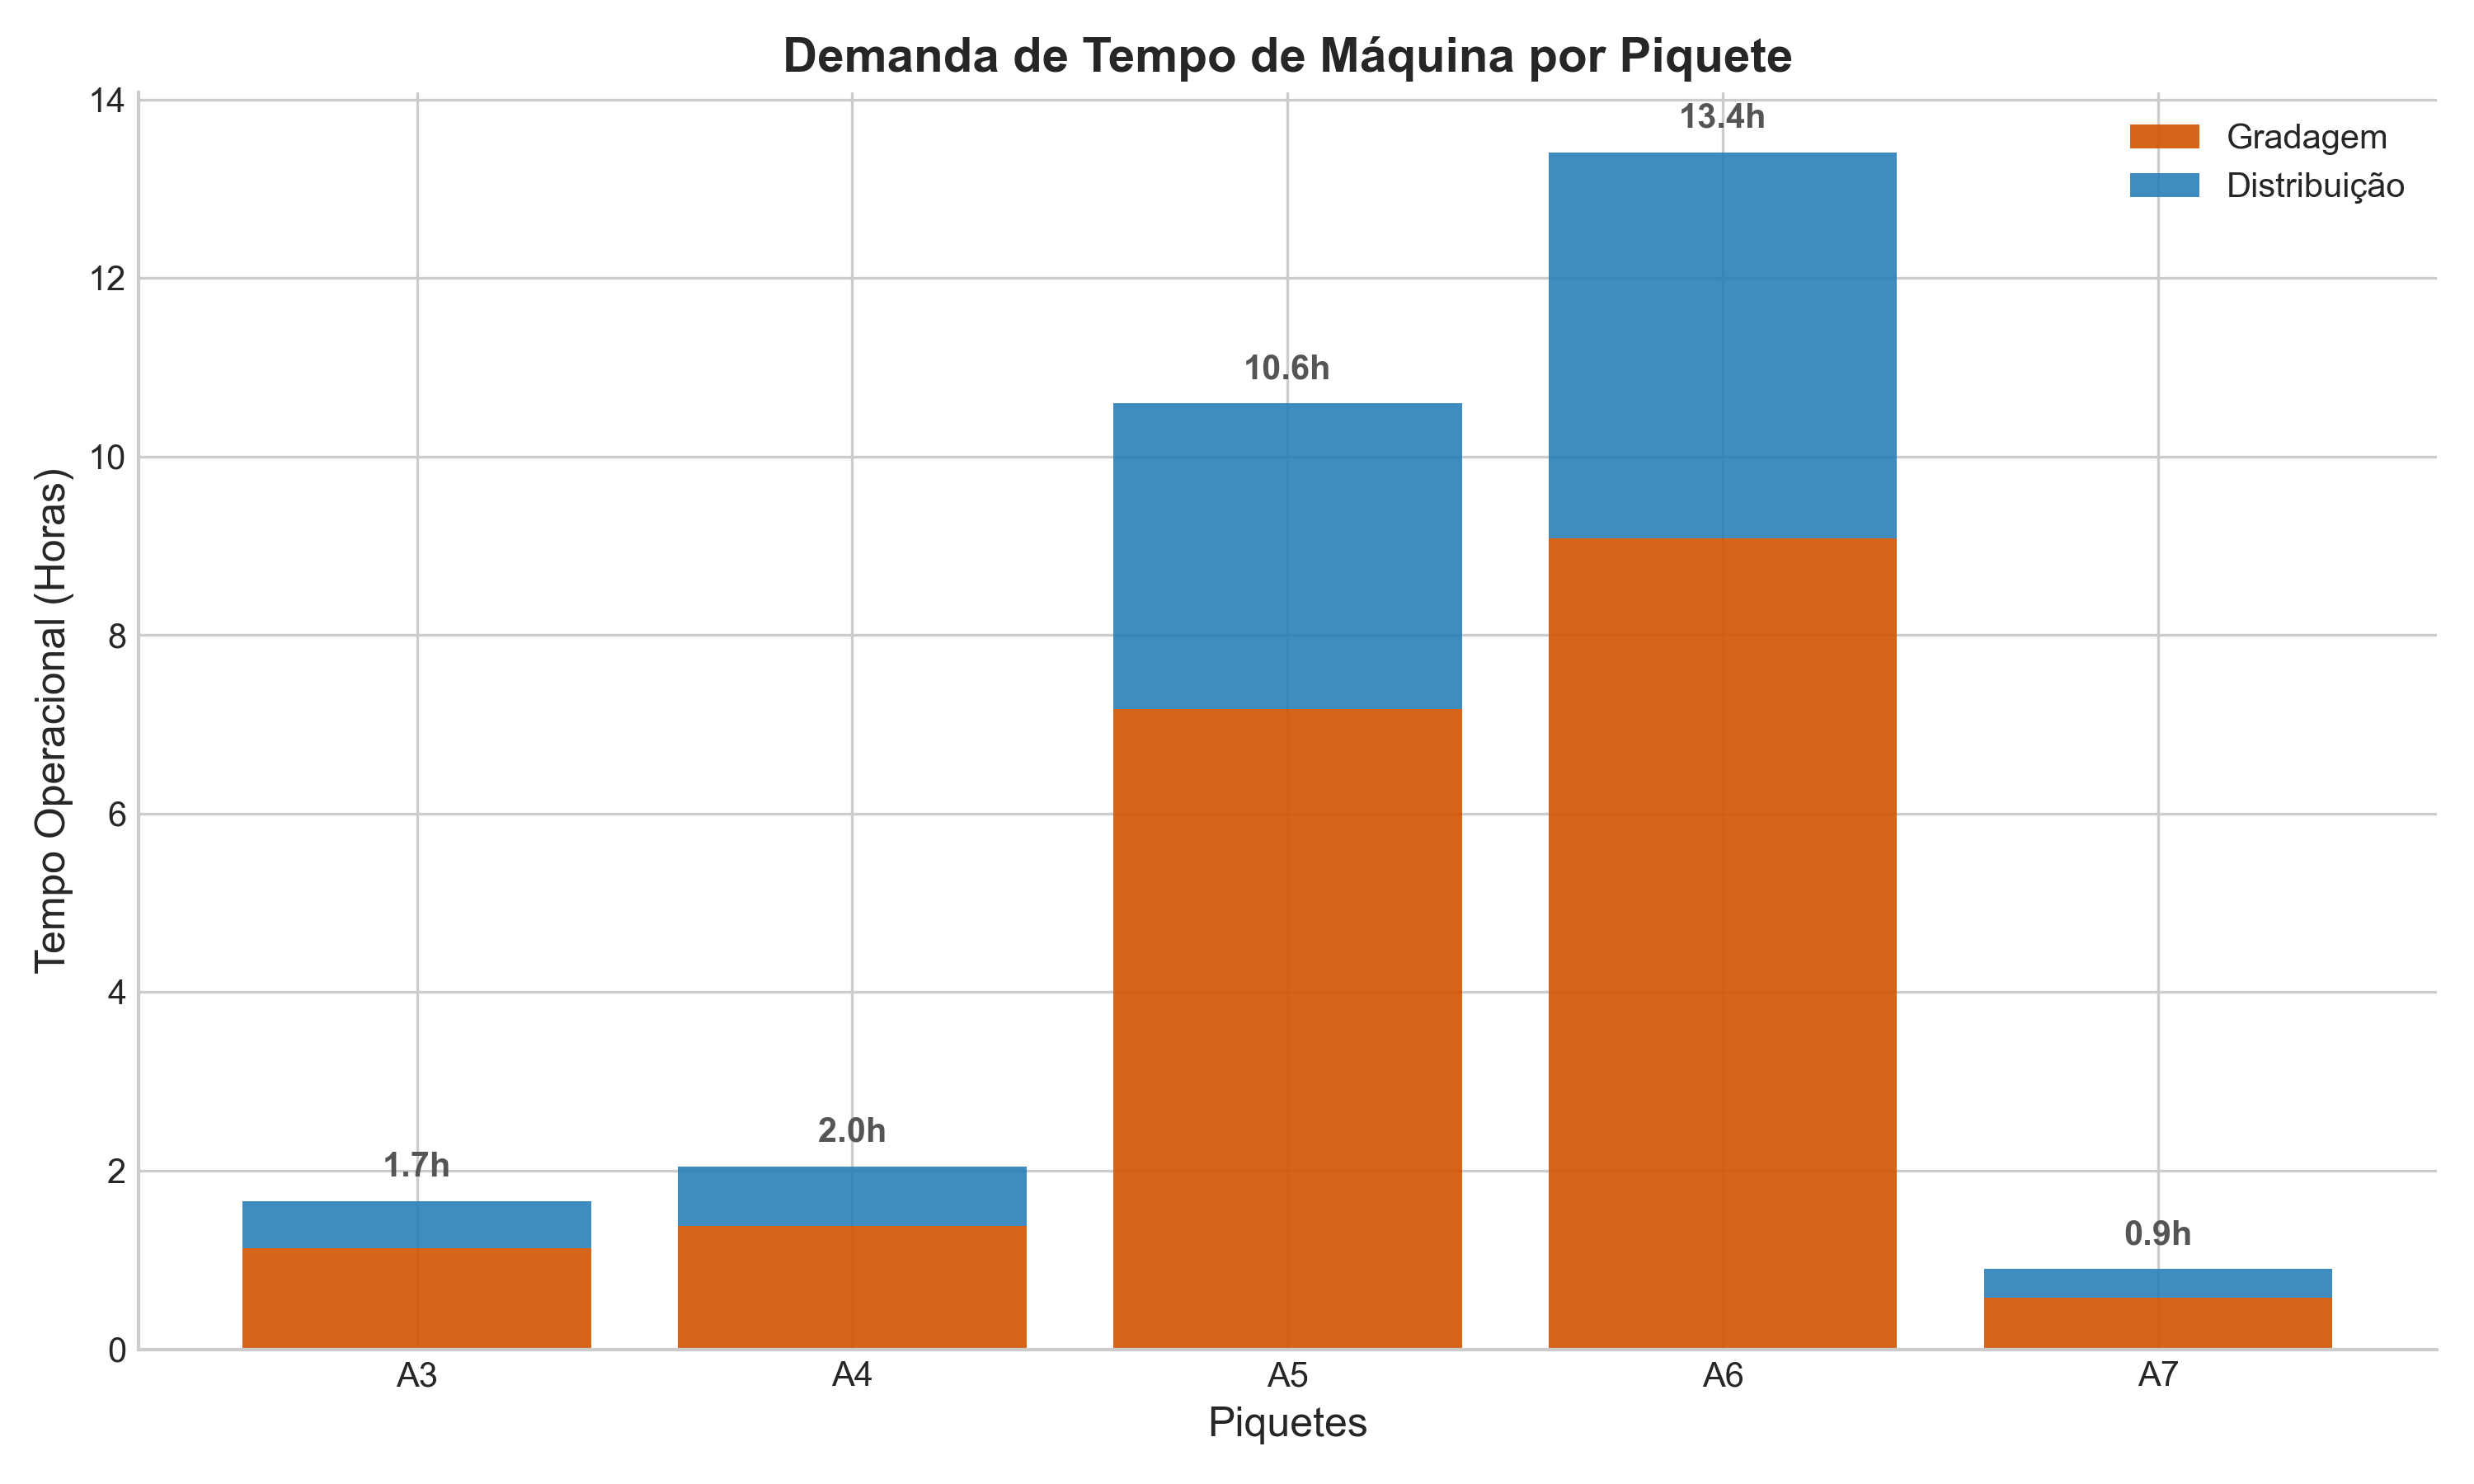
\includegraphics[width=0.9\textwidth]{grafico_tempo_por_piquete.png}

\begin{minipage}{0.9\textwidth}
    \setlength{\parindent}{1em}
    \raggedright
    Fonte: Elaborado pelos autores (2025)
\end{minipage}

\end{figuraabnt}


\section{Análise de consumo energético}

O consumo de combustível é um dos principais componentes do custo variável do trator. Para a estimativa, utilizou-se o consumo horário médio aferido de 9,0 L/h. O ciclo completo de reforma de pastagem envolve:
\begin{enumerate}
    \item \textbf{Preparo Primário:} 1ª Gradagem (rompimento superficial);
    \item \textbf{Semeadura:} Distribuição a lanço;
    \item \textbf{Incorporação:} 2ª Gradagem (leve);
    \item \textbf{Adubação:} Aplicação de cobertura.
\end{enumerate}

A Tabela \ref{tab:consumo_diesel} detalha a demanda de diesel para reformar integralmente cada piquete.

\begin{table}[H]
    \centering
    \caption{Demanda energética total (óleo diesel) para reforma completa.}
    \label{tab:consumo_diesel}
    \vspace{0.1cm}
    \begin{tabular}{cccc}
        \toprule
        \textbf{Piquete} & \textbf{Área (ha)} & \textbf{Tempo de Ciclo Total (h)\textsuperscript{*}} & \textbf{Consumo Diesel (L)} \\
        \midrule
        A3 & 1,8 & 3,33 & \textbf{30,0} \\
        A4 & 2,2 & 4,10 & \textbf{36,9} \\
        A5 & 11,2 & 21,20 & \textbf{190,8} \\
        A6 & 14,2 & 26,83 & \textbf{241,5} \\
        A7 & 0,8 & 1,80 & \textbf{16,2} \\
        \midrule
        \textbf{Total} & \textbf{30,2} & \textbf{57,26} & \textbf{515,4} \\
        \bottomrule
    \end{tabular}
    \begin{flushleft}\begin{footnotesize}
       Fonte: Autores (2025). \textsuperscript{*}Soma dos tempos de 2 passadas de grade e 2 de distribuição.
    \end{footnotesize}\end{flushleft}
\end{table}

A demanda energética é um indicador crítico para o planejamento econômico da propriedade, pois o custo do combustível representa uma parcela significativa dos custos operacionais. A Figura \ref{fig:diesel} apresenta de forma visual a distribuição do consumo de diesel necessário para a reforma completa de cada piquete, considerando o ciclo integral de operações (duas passadas de gradagem e duas de distribuição). Este gráfico permite identificar rapidamente quais piquetes demandam maior investimento energético e facilita o planejamento de compra de insumos e disponibilidade de capital de giro durante as épocas críticas de plantio.

%figura grafico diesel
\begin{figuraabnt}{Consumo diesel}{fig:diesel}
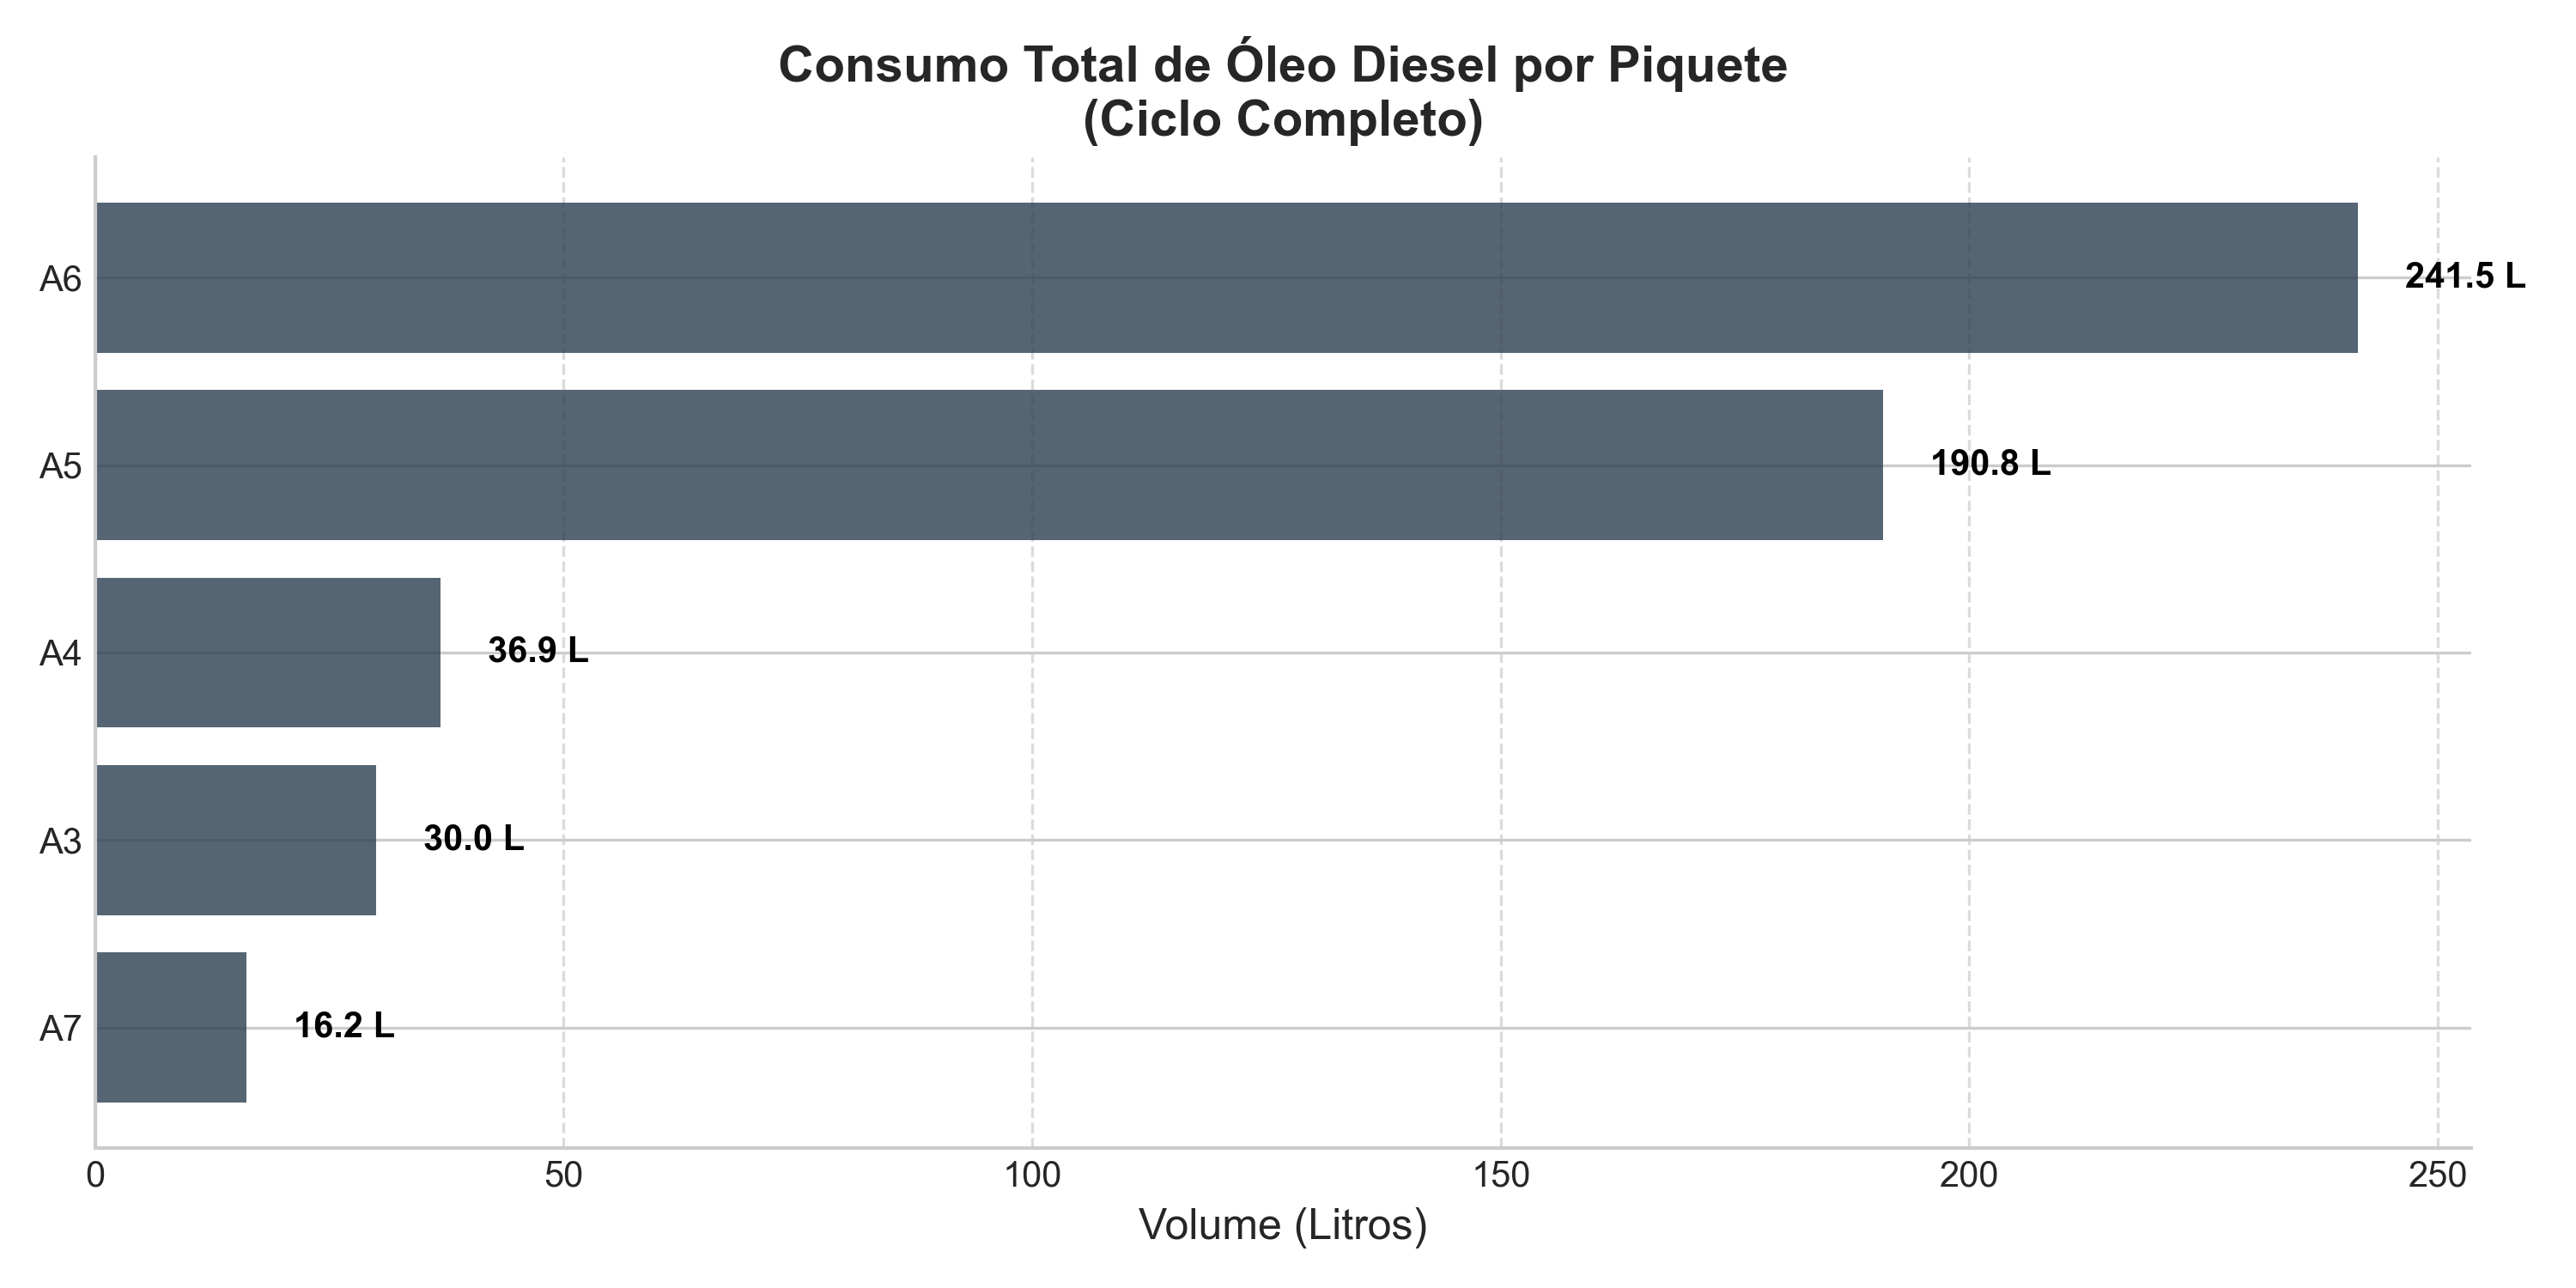
\includegraphics[width=0.9\textwidth]{grafico_consumo_diesel.png}

\begin{minipage}{0.9\textwidth}
    \setlength{\parindent}{1em}
    \raggedright
    Fonte: Elaborado pelos autores (2025)
\end{minipage}

\end{figuraabnt}
Os resultados indicam que para a reforma completa dos 30,2 hectares analisados, serão necessárias aproximadamente 57 horas de trabalho de máquina e 515 litros de diesel. Estes dados permitem ao produtor planejar a compra de insumos e a disponibilidade de mão de obra nas janelas de plantio.


\section{Diagnóstico da mecanização em relação à atividade produtiva}

A análise do parque de máquinas da Fazenda Canoas indica um nível de mecanização compatível com o sistema de preparo periódico do solo adotado para a renovação de pastagens. A frota de tratores, com potências de 75 cv e 103 cv, encontra-se adequadamente dimensionada para tracionar os implementos de preparo secundário (grades de 28 discos) e distribuição a lanço, respeitando a reserva de potência necessária para solos argilosos e topografia ondulada, conforme preconizado por \citeonline{bauer2019p1} para evitar sobrecargas no motor e na transmissão.

Entretanto, do ponto de vista agronômico, o diagnóstico aponta para uma dependência excessiva da grade niveladora como implemento único de preparo. Segundo, embora as grades ofereçam maior capacidade operacional em relação aos arados, seu uso continuado à mesma profundidade (limitada a cerca de 15 a 20 cm) favorece a formação da camada compactada subsuperficial conhecida como ``pé-de-grade''. No contexto da atividade produtiva da fazenda (pecuária), essa compactação é agravada pelo pisoteio animal, podendo limitar o desenvolvimento radicular das pastagens e a infiltração de água. Portanto, embora o conjunto mecanizado seja eficiente operacionalmente (atendendo à janela de plantio de 57 horas calculada), ele requer monitoramento técnico para evitar a degradação física do solo a médio prazo.




\chapter{Considerações finais}

O diagnóstico da mecanização na Fazenda Canoas revela um parque de máquinas dimensionado adequadamente para a escala produtiva atual, com independência financeira na aquisição dos bens. A frota, composta por dois tratores (103 cv e 75 cv), atende com folga a demanda de potência para os implementos de preparo secundário (grades de 28 discos) e distribuição a lanço identificados no inventário.

A análise operacional indicou que a reforma completa dos 30,2 hectares de pastagens demanda aproximadamente 57,26 horas de trabalho e um consumo estimado de 515 litros de diesel. Este dado é crucial para o planejamento da propriedade, pois permite prever que, com apenas um operador e um trator principal, a janela de plantio necessária é de aproximadamente uma semana de trabalho (considerando jornadas de 8h e as eficiências de campo calculadas neste estudo).

Entretanto, observa-se que o sistema produtivo baseia-se exclusivamente no uso de grades (preparo periódico). Embora eficaz para a incorporação de sementes a lanço, este método apresenta riscos de degradação física do solo a longo prazo. O uso contínuo de grades na mesma profundidade pode levar à formação de camadas compactadas subsuperficiais, conhecidas tecnicamente como ``pé-de-grade'', que dificultam a infiltração de água e o crescimento radicular (\citeonline{bauer2019p1}).

Recomenda-se, como melhoria futura, a avaliação técnica para a introdução de um escarificador para descompactação eventual ou a transição gradual para o Sistema de Plantio Direto na Palha (SPDP) em áreas declivosas. Segundo \citeonline{bauer2019p1}, tais práticas visam a conservação do solo e a redução do consumo energético, uma vez que o preparo convencional demanda maior revolvimento e potência. A manutenção preventiva rigorosa deve ser mantida, visto que os custos variáveis (combustível e reparos) representam a maior parcela do custo horário atual, já que o custo fixo de aquisição foi amortizado.


\bibliography{bibliografia}
\end{document}
